\documentclass[english]{report}
\usepackage{graphicx}
\usepackage{booktabs}
\usepackage{geometry}
\usepackage{hyperref}
\usepackage{babel}
\usepackage{lipsum}
\usepackage{subcaption}
\usepackage{float}
\usepackage{colortbl}
\usepackage{amsmath}
\usepackage{amssymb}

 \geometry{
 a4paper,
 total={170mm,257mm},
 left=20mm,
 top=20mm,
 }

\title{
    \leavevmode{
\includegraphics[width=1\textwidth]{../resources/img/polito_logo_2021_blu}\newline\newline}\\
     Fingerprint spoofing detection \\

}
\author{Riccardo Cardona, Nicholas Berardo}

\begin{document}

\maketitle
\tableofcontents

\chapter{Introduction}

\section{Abstract}
    The goal is to build the best model for the Fingerprint-Spoofing Detection task, using the models developed during the
    laboratory and the lessons.

\section{Overview}
    The data set and test set are composed of 10 dimensional features.
    The last column is the class label which is \textbf{1} for the \textit{authentic fingerprint} and \textbf{0} for the \textit{spoofed fingerprint}.\newline

    The datasets are imbalanced, we have more spoofed fingerprint than the authentic fingerprint.
    The Training set is composed of 2325 samples and the Test set is composed of 7704 samples. \newline

    The application we are going to build has $\pi$ =0.5 meaning that we have the same prior probability for both classes, but we have different costs.
    The cost of False Negative \textit{C\textsubscript{fn}} is 1 but the cost of False Positive
    \textit{C\textsubscript{fp}} is 10, so classifying a spoofed fingerprint as an authentic one
    has an higher cost due to security vulnerability.

\section{Features Analisys}
As we said, the Fingerprint Spoofing Detection task has 10 features.
Here below we are going to analyze them.

\begin{figure}[h!]
    \begin{subfigure}{0.3\textwidth}
        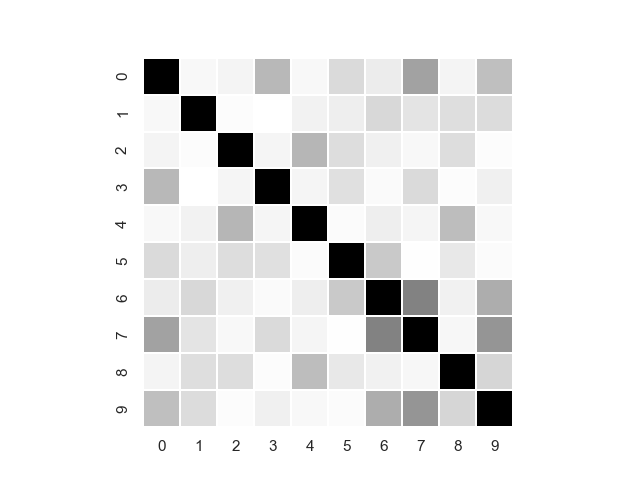
\includegraphics[scale=0.3]{../../images/feature_plot/heatmap_}
        \caption{All classes}

    \end{subfigure}
    \begin{subfigure}{0.3\textwidth}
        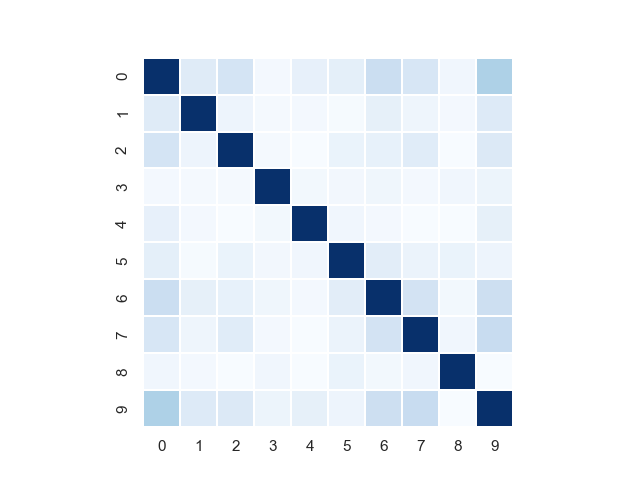
\includegraphics[scale=0.3]{../../images/feature_plot/heatmap_fingerprint_}
        \caption{Authentic Fingerprint}

    \end{subfigure}
    \begin{subfigure}{0.3\textwidth}
        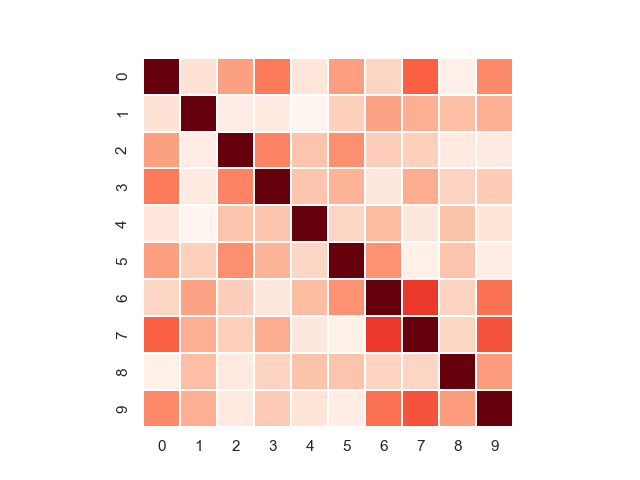
\includegraphics[scale=0.3]{../../images/feature_plot/heatmap_spoofedFingerprint_}
        \caption{Spoofed Fingerprint}

    \end{subfigure}
    \centering
    \caption{Heatmap}
    \label{fig:HeatMap}
\end{figure}

As we can see from the Figure~\ref{fig:HeatMap}, the correlation between the features is very small.
This lead us to think that using PCA for dimensionality reduction is useless (it could
also remove some important information!), but we will try using it. \newline

Now we are going to see the histograms for each of the 10 features.
It's easy to see that each feature has a Gaussian distribution. \newline

\begin{figure}[h!]
    \begin{subfigure}{0.3\textwidth}
        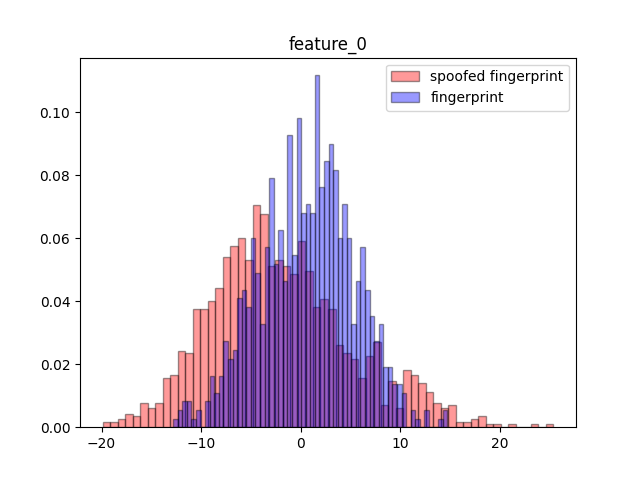
\includegraphics[scale=0.3]{../../images/feature_plot/hist_feature_0}
        \caption{RAW Feature 0}
    \end{subfigure}
    \begin{subfigure}{0.3\textwidth}
        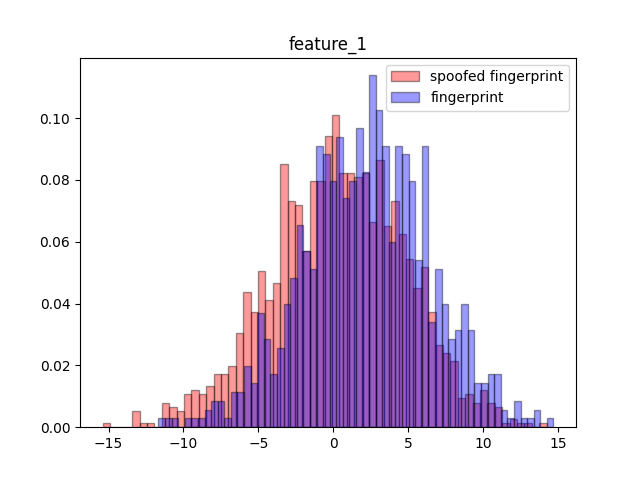
\includegraphics[scale=0.3]{../../images/feature_plot/hist_feature_1}
        \caption{RAW Feature 1}
    \end{subfigure}
    \begin{subfigure}{0.3\textwidth}
        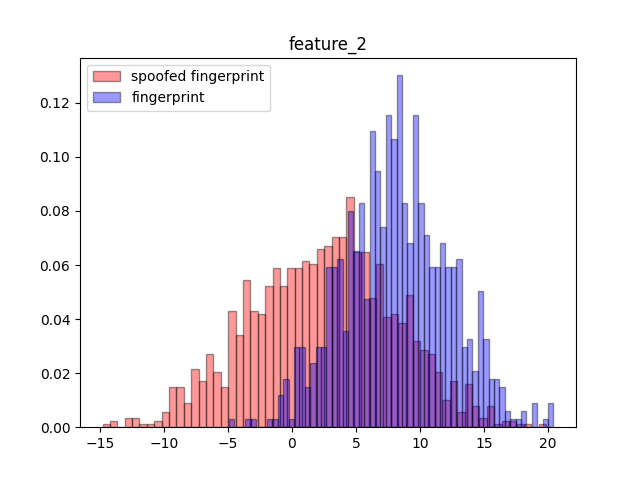
\includegraphics[scale=0.3]{../../images/feature_plot/hist_feature_2}
        \caption{RAW Feature 2}
    \end{subfigure}
    \begin{subfigure}{0.3\textwidth}
        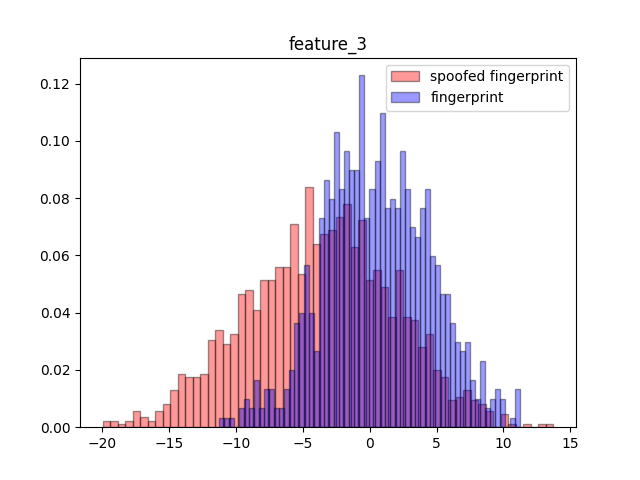
\includegraphics[scale=0.3]{../../images/feature_plot/hist_feature_3}
        \caption{RAW Feature 3}
    \end{subfigure}
    \begin{subfigure}{0.3\textwidth}
        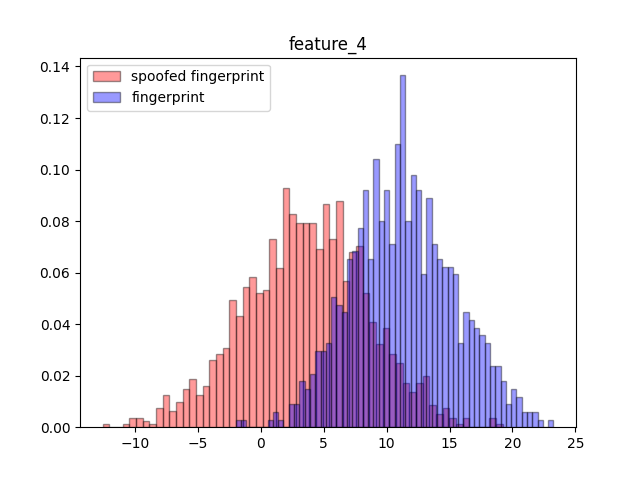
\includegraphics[scale=0.3]{../../images/feature_plot/hist_feature_4}
        \caption{RAW Feature 4}
    \end{subfigure}
    \begin{subfigure}{0.3\textwidth}
        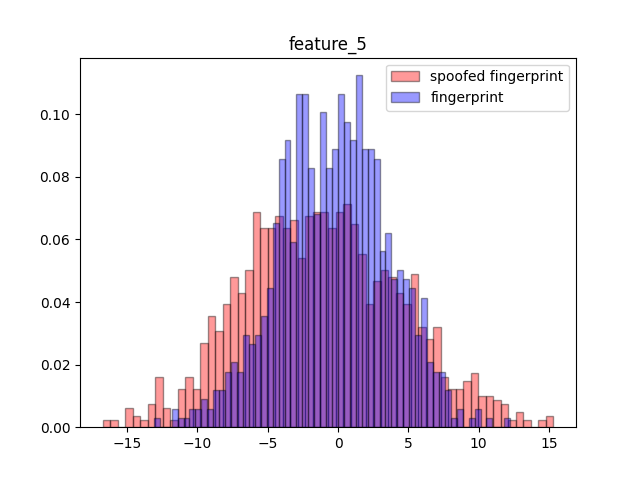
\includegraphics[scale=0.3]{../../images/feature_plot/hist_feature_5}
        \caption{RAW Feature 5}
    \end{subfigure}
    \begin{subfigure}{0.3\textwidth}
        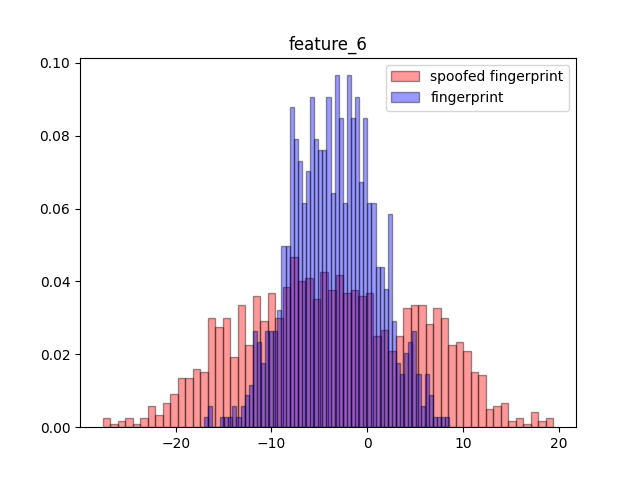
\includegraphics[scale=0.3]{../../images/feature_plot/hist_feature_6}
        \caption{RAW Feature 6}
    \end{subfigure}
    \begin{subfigure}{0.3\textwidth}
        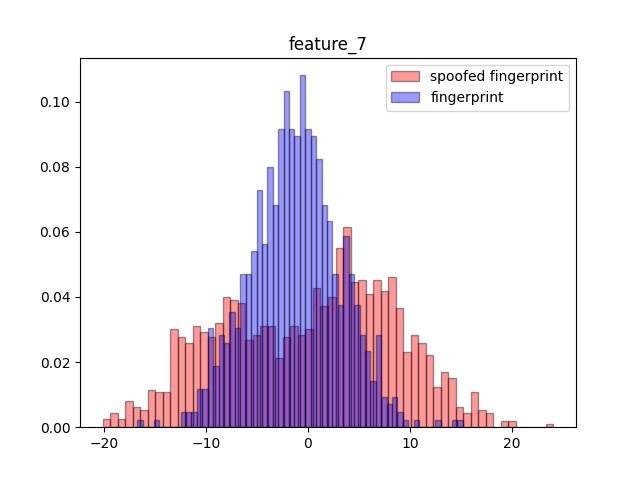
\includegraphics[scale=0.3]{../../images/feature_plot/hist_feature_7}
        \caption{RAW Feature 7}
    \end{subfigure}
    \begin{subfigure}{0.3\textwidth}
        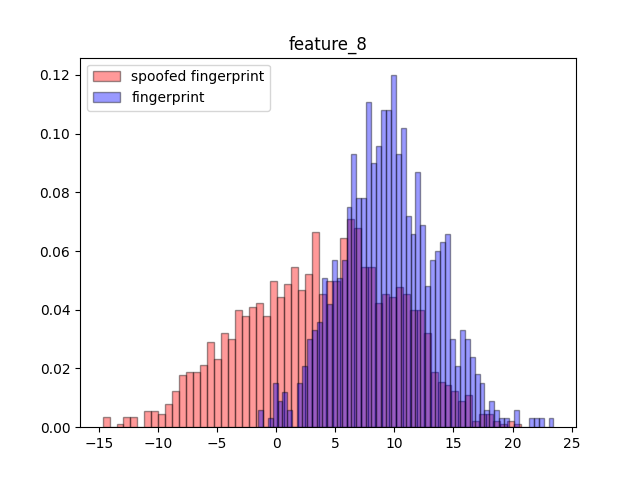
\includegraphics[scale=0.3]{../../images/feature_plot/hist_feature_8}
        \caption{RAW Feature 8}
    \end{subfigure}
    \begin{subfigure}{0.3\textwidth}
        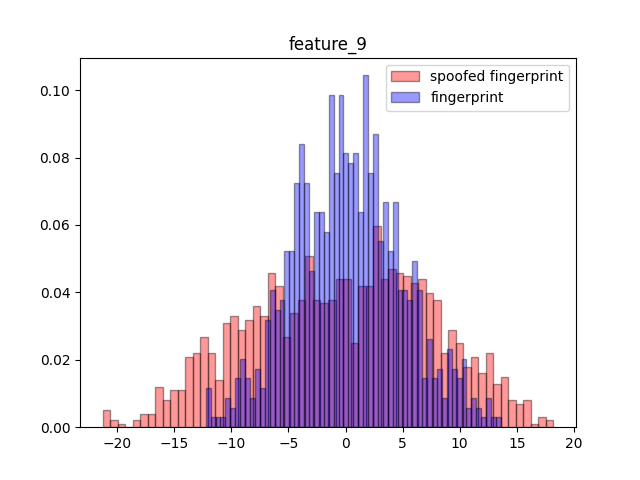
\includegraphics[scale=0.3]{../../images/feature_plot/hist_feature_9}
        \caption{RAW Feature 9}
    \end{subfigure}
    \centering
    \caption{RAW Feature Histogram}
    \label{fig:RawFeatureHistogram}
\end{figure}


\section{PCA Usage}

    PCA (Principal Component Analysis) is a Dimensionality Reduction technique that can be used to
    remove noise, simplify classification and data visualization.
    It can be also used to avoid overfitting, but it may produce underfitting if too many dimensions are removed
    (removing too much useful information).
    So it is a useful technique, but sometimes it can be useless because if used could
    lead only to bad models. \newline\newline
    What does PCA do? 

    First of all we need to compute the mean of the Dataset $\mu$, then we need to compute the covariance
    matrix
    \[C = \frac{1}{K} \sum_{i=1}^{K} (x_i-\mu)(x_i-\mu)^T \]
    From C we need the eigen-decomposition \(C = U \Sigma U^T \), where U is a matrix that
    contains the eigen-vectors and $\Sigma$ is a diagonal matrix that contains the eigen-values
    in descending order.
    The solution are the \textit{m} eigen-vectors of U corresponding to the \textit{m}
    highest eigen-values of $\Sigma$.

    \begin{figure}[H]
        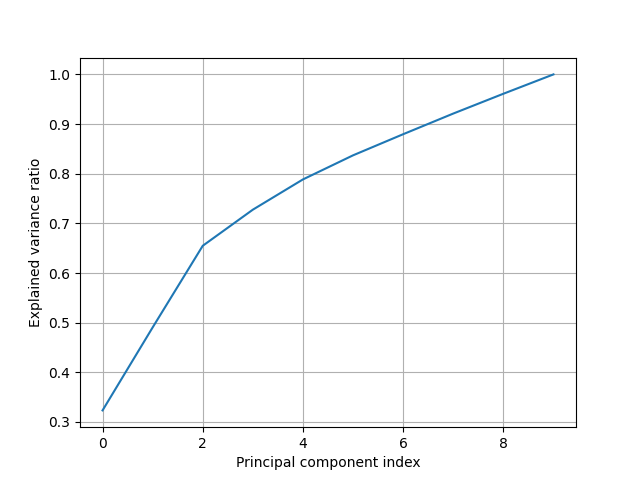
\includegraphics[scale=0.5]{../../images/feature_plot/PCA_explainedVariance}
        \centering
        \caption{PCA variance}
        \label{fig:PCAvariance}
    \end{figure}

    As we can see, if we use 9 dimensions (Number 8 on the principal component index), we are going to
    reach a 96\% of explainance, then if we use 8 dimensions we will explain 91\% of the data variance.
    Starting from 7 to 1 dimensions, we are lower than 90\%. \newline
    We will consider only 9 and 8 as PCA parameter.

    \begin{figure}[H]
        \centering
        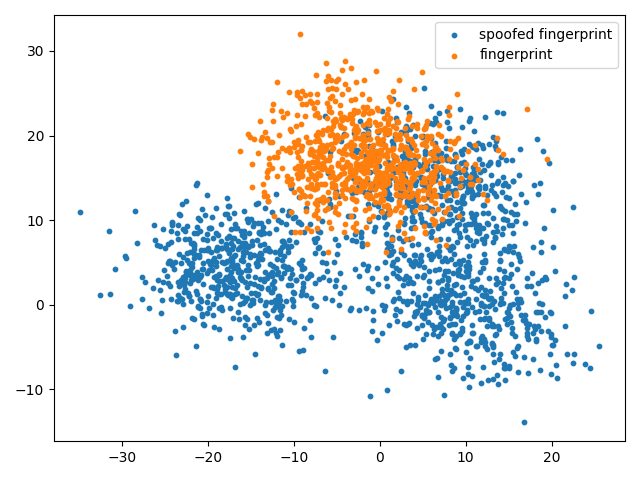
\includegraphics[scale=0.5]{../../images/feature_plot/PCA_m=2}
        \caption{PCA}
        \label{fig:PCA}
    \end{figure}

    From this plot (Figure~\ref{fig:PCA}) we can see the distribution of the 2 main features.
    It's also easy to see that linear models won't be able to find a separation, meanwhile the quadratic models will find a separation.
    So models like MVG, Quadratic SVM and RBF SVM will perform well.

    \begin{figure}[H]
        \centering
        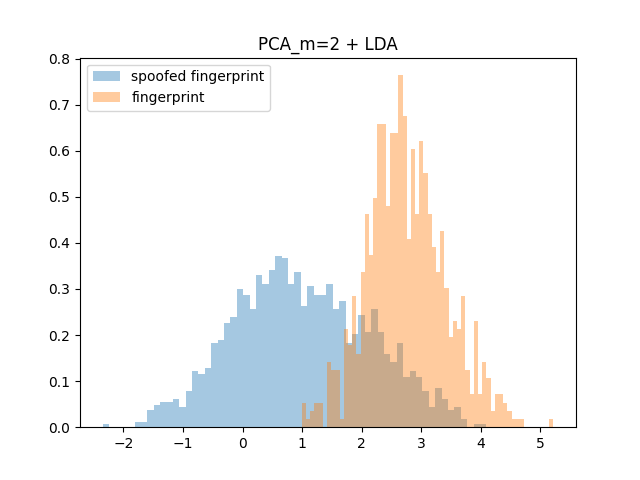
\includegraphics[scale=0.5]{../../images/feature_plot/histPCA_m=2 + LDA}
        \caption{LDA}
        \label{fig:LDA}
    \end{figure}

    From this plot (Figure~\ref{fig:LDA}) we can see the distribution of the 2 main features using both PCA and LDA

\section{Training}
    \begin{itemize}
        \item We are going to use a K-Fold Cross Validation approach, with K = 5
        \item The minDCF computation is computed based on our application ($\pi$,C\textsubscript{fn},C\textsubscript{fp}) = (0.5,1,10), but we have
        computed the effective prior, which is approximated to ($\pi$,C\textsubscript{fn},C\textsubscript{fp}) = (0.09,1,1).\newline
        We have also tried this two different application:
        \begin{itemize}
            \item ($\pi$,C\textsubscript{fn},C\textsubscript{fp}) = (0.1,1,1)
            \item ($\pi$,C\textsubscript{fn},C\textsubscript{fp}) = (0.9,1,1)
        \end{itemize}
    \end{itemize}

\chapter{Classification and Validation}

\section{Introduction}
We are going to develop this following models:
\begin{itemize}
    \item Generative Models
    \begin{itemize}
        \item Multivariate Gaussian Classifier (\textbf{MVG})
        \item MVG Tied Covariance (Only one covariance matrix for everything)
        \item MVG Naive (For each covariance matrix takes out only the diagonal)
        \item MVG Tied Naive (Only one covariance matrix, but taking only the diagonal)
    \end{itemize}
    \item Logistic Regression (\textbf{LR})
    \begin{itemize}
        \item Linear Logistic Regression
    \end{itemize}
    \item Support Vector Machine (\textbf{SVM})
    \begin{itemize}
        \item Linear SVM
        \item Polynomial SVM
        \item Radial Basis Function SVM
    \end{itemize}
    \item Gaussian Mixture Models (\textbf{GMM})
    \begin{itemize}
        \item Full Covariance Matrix
        \item Diagonal Covariance Matrix
        \item Tied Full Covariance Matrix
        \item Tied Diagonal Covariance Matrix
    \end{itemize}
\end{itemize}

\clearpage

\section{Multivariate Gaussian Classifiers}

We are going to analyze all the Gaussian Classifiers, using the Multivariate Gaussian Classifier and all it's variants: 
\begin{itemize}
    \item Tied Covariance
    \item Naive Bayes
    \item Tied Naive Bayes
\end{itemize}

For all these 4 models we have 2 parameters: $\theta$ = ($\mu$, $\Sigma$). We can easily estimate them starting
from the likelihood w.r.t. $\theta$ for the \textbf{M.V.G.}
\[ \mathcal{L} (\theta) = \prod_{c}^{K}\prod_{i|c_i=c} \mathcal{N} (x_i|\mu_c,\Sigma_c)\]
Then we can build the log-likelihood because it's easier to work with.
\[ l (\theta) = \sum_{c}^{K}\sum_{i|c_i=c} \log \mathcal{N} (x_i|\mu_c,\Sigma_c)\]
Now we define \( l_c (\theta) = \sum_{i|c_i=c} \log \mathcal{N} (x_i|\mu_c,\Sigma_c)\) and compute
the $\nabla_\mu l_c(\mu_c,\Sigma_c) = 0$ and the $\nabla_\Sigma l_c(\mu_c,\Sigma_c) = 0$ 
obtaining 
\[\mu_c^* = \frac{1}{N_c}\sum_{i|c_i=c}x_i\]
\[\Sigma_c^* = \frac{1}{N_c}\sum_{i|c_i=c}(x_i-\mu_c^*)(x_i-\mu_c^*)^T\]
We can do the same thing for the \textbf{Naive Bayes} model (that has diagonal covariance matrix)
\[ l (\theta) = \sum_{c}^{K}\sum_{i|c_i=c}\sum_{j=1}^{D} \log \mathcal{N} (x_{i,[j]}|\mu_{c,[j]},\Sigma_{c,[j]})\]
which solutions are
\[\mu_{c,[j]}^* = \frac{1}{N_c}\sum_{i|c_i=c}x_{i,[j]}\] 
\[\Sigma_{c,[j]}^* = \frac{1}{N_c}\sum_{i|c_i=c}(x_{i,[j]}-\mu_{c,[j]}^*)(x_{i,[j]}-\mu_{c,[j]}^*)^T\] 

Finally, the \textbf{Tied} model can be built in the same way (has a single covariance matrix for all classes)
\[ l (\theta) = \sum_{c}^{K}\sum_{i|c_i=c} \log \mathcal{N} (x_i|\mu_c,\Sigma)\]
which solutions are
\[\mu_{c}^* = \frac{1}{N_c}\sum_{i|c_i=c}x_{i}\] 
\[\Sigma^* = \frac{1}{N}\sum_{c}^{K}\sum_{i|c_i=c}(x_{i}-\mu_{c}^*)(x_{i}-\mu_{c}^*)^T\] 

The tables below show the computation of the minDCF on the validation set (extracted using K-Fold Cross Validation with K = 5).
As said before, we are going to consider the main application (0.5,1,10) and 2 other applications (0.1,1,1) and (0.9,1,1).
There are also some computation of PCA with m=9 and m=8.

\begin{table}[H]
    \centering
    \begin{tabular}{@{}llll@{}}
    \toprule
    Classifier          & pi = 0.1  & pi = 0.5  & pi = 0.9 \\ \midrule
                        & \multicolumn{3}{c}{RAW Features - NO PCA} \\ \midrule
    MVG                 & 0.616     & \color{red}{0.331}     & 0.111    \\
    Naive Gaussian      & 0.806     & 0.472     & 0.144    \\
    Tied Gaussian       & 0.706     & 0.486     & 0.184    \\
    Naive Tied Gaussian & 0.79      & 0.551     & 0.198    \\ \bottomrule
    \end{tabular}
    \label{tab:MVG_RAW_valid}
\end{table}

\begin{table}[H]
    \centering
    \begin{tabular}{@{}lllllll@{}}
    \toprule
    Classifiers         & pi = 0.1 & pi = 0.5 & pi = 0.9 \\ \midrule
                        & \multicolumn{3}{c}{PCA (m=9)}  \\ \midrule
    MVG                 & 0.629    & \color{red}{0.33}    & 0.109    \\
    Naive Gaussian      & 0.74    & 0.369    & 0.113    \\
    Tied Gaussian       & 0.696    & 0.492    & 0.18    \\
    Naive Tied Gaussian & 0.772    & 0.543    & 0.202    \\ \bottomrule
    \end{tabular}
    \label{tab:MVG_PCA9_valid}
\end{table}

\begin{table}[H]
    \centering
    \begin{tabular}{@{}lllllll@{}}
    \toprule
    Classifiers         & pi = 0.1 & pi = 0.5 & pi = 0.9 \\ \midrule
                        & \multicolumn{3}{c}{PCA (m=8)}  \\ \midrule
    MVG                 & 0.612    & \color{red}{0.333}    & 0.109    \\
    Naive Gaussian      & 0.712     & 0.36    & 0.112    \\
    Tied Gaussian       & 0.686    & 0.485    & 0.181    \\
    Naive Tied Gaussian & 0.774    & 0.544    & 0.201    \\ \bottomrule
    \end{tabular}
    \label{tab:MVG_PCA8_valid}
\end{table}

As we can see, the MVG model, that consider all the covariance matrices, is the best either with PCA or without.
As we said previously, the quadratic models do a good job on these data, in fact the MVG is the best, meanwhile the Tieds are the worst.
PCA is useful only in the Naive Gaussian model.
Tied models perform worse.

Overall the best candidate is the \textbf{MVG classifier} without PCA. However, we will see that this kind of model is also
useless for our imbalanced data.

\clearpage

\section{Logistic Regression}

We are going to analyze both Linear Logistic Regression and Quadratic Logistic Regression.
\subsection{Linear Logistic Regression}

Logistic Regression is a discriminative model that directly computes the posterior probability \(P(C=c|X=x)\).
The model parameters are (w,b) that can be estimated using a frequentist approach.
There's also an hyper-parameter $\lambda$ that must be estimated by cross-validation. $\lambda$ is needed to avoid overfitting, if it's too high then the model will
underfit but if it's too low then the model will overfit.\newline

The plots show how minDCF is affected by different values of $\lambda$.
They are exploited to calibrate $\lambda$, which is the regularization coefficient.

\begin{figure}[H]
    \centering
    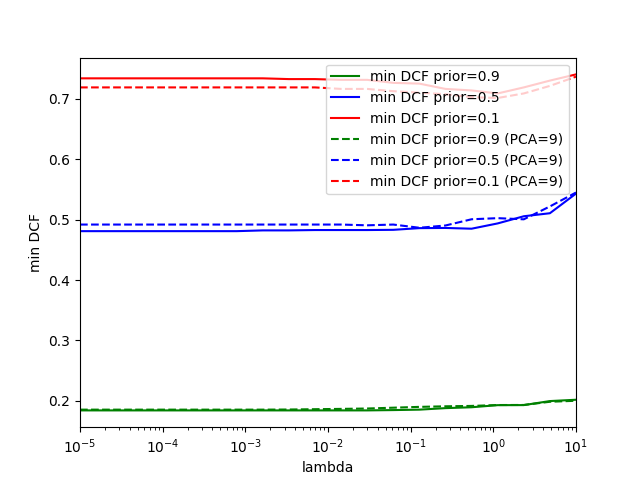
\includegraphics[scale=0.5]{../../images/validation/LR_PCA_minDCF_comparison}
    \caption{DCF - Linear LogReg}
    \label{fig:DCF_LinearLogReg_valid}
\end{figure}

The Figure~\ref{fig:DCF_LinearLogReg_valid} shows that using a $\lambda$ = 10\textsuperscript{-5} or $\lambda$ = 10\textsuperscript{-1}
is more or less the same, the minDCF doesn't change that much.
From $\lambda$ = 10\textsuperscript{-1} to +$\infty$ the minDCF will be too high.

For our main application, it's hard to see, but $\lambda$ = 0.4 is the best choice. By the way, the LR computes a linear separation,
but we said that the separation can't be found using a linear function, so we expect higher minDCF than the MVG.

\begin{table}[H]
    \centering
    \begin{tabular}{lllllll}
        \toprule
                                & pi=0.1 & pi=0.5 & pi=0.9 \\ \midrule
                                & \multicolumn{3}{c}{NO-PCA}  \\
    Log Reg ($\lambda$ = 0.4)   & 0.715      & 0.485      & 0.189  \\ \midrule
                                & \multicolumn{3}{c}{PCA m=9}  \\
    Log Reg ($\lambda$ = 0.4)   & 0.705      & 0.496       & 0.193 \\ \midrule
                                & \multicolumn{3}{c}{PCA m=8}  \\
    Log Reg ($\lambda$ = 0.4)   & 0.689       & \color{red}{0.483}       & 0.188 \\
    \bottomrule
    \end{tabular}
    \label{tab:LinearLogReg_valid}
\end{table}

Overall, the MVG without PCA has a \textbf{minDCF = 0.331} and this value is better than all
the Linear Logistic Regression values (for our main application).

\clearpage

\section{Support Vector Machine}

In this section we are going to see how Linear SVM, Polynomial SVM and RBF SVM will handle our application.
$\newline$

\textbf{SVM - Linear}

$\newline$
\textbf{Linear SVM} can be obtained by the minimization of the primal problem:
\[\hat{J}(\hat{w}) = \frac{1}{2}||\hat{w}||^2 + C\sum_{i=1}^{n}max_i(0,1-z_i(\hat{w}^T\hat{x_i}))\]
where
\[\hat{x_i} = \biggl[ \hat{x_i} K \biggr] , \hat{w_i} = \biggl[w b\biggr]\]
and K is a regularization term.
\begin{figure}[h!]
    \centering
    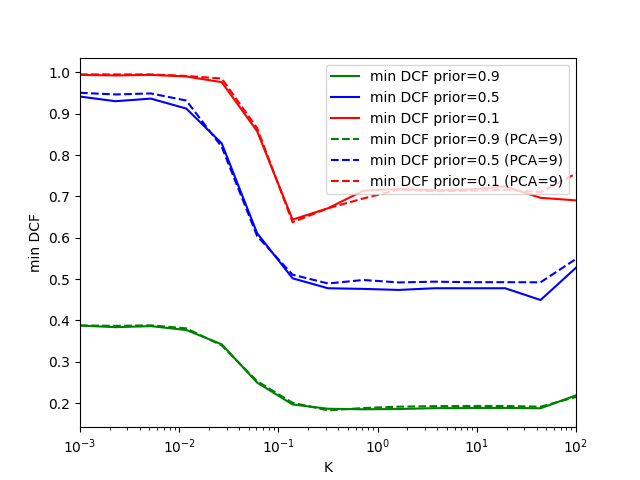
\includegraphics[scale = 0.5]{../../images/validation/SVM_minDCF_comparison_C=1}
    \caption{Linear SVM with C=1}
    \label{fig:LinearSVM_C1_valid}
\end{figure}

From Figure~\ref{fig:LinearSVM_C1_valid} we can see how K is affected (using C = 1).
It can be seen that values of K between $10^{-1}$ and $10^{1}$ have a low DCF. In our cases we are going to try 3 different
values of \(K = [0.1, 1, 10]\).

\begin{figure}[h!]
    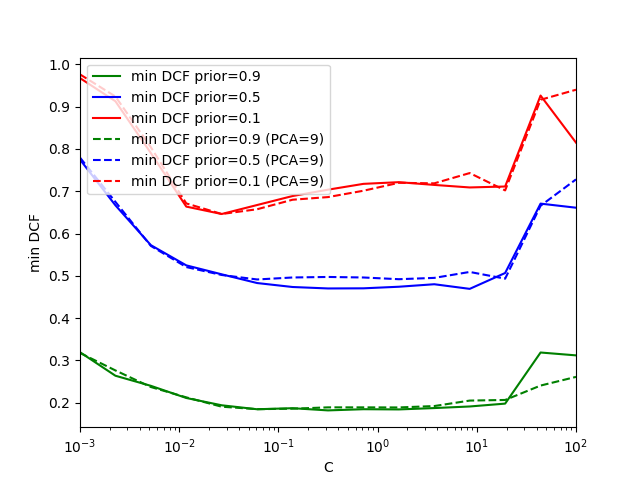
\includegraphics[scale = 0.5]{../../images/validation/SVM_minDCF_comparison_K=1}
    \centering
    \caption{Linear SVM with K=1}
    \label{fig:LinearSVM_K1_valid}
\end{figure}

Figure~\ref{fig:LinearSVM_K1_valid} shows the different values of C while setting K = 1.
Again, it can be seen that the optimal values of C are the ones between $10^{-1}$ and $10^{1}$.
We are going to test 4 different values of \(C = [0.01, 0.1, 1, 10]\).
We also decided to test 0.01 even if the minDCF is \("\)optimal\("\) only for the $\pi$ = 0.1

Here the table containing the results:

$\newline$
\textbf{SVM - Linear - RAW Featues}
\begin{table}[H]
    \centering
    \begin{tabular}{ll|lllll}
        \hline
                                & &         K = 0.1 & K = 1.0 & K = 10 \\ \hline
                                & & \multicolumn{3}{c}{$\pi$=0.1} \\ \hline
                                & C = 0.01   & 0.99 & 0.68 & 0.71   \\
                                & C = 0.1    & 0.964 & 0.672 & 0.713  \\
                                & C = 1.0    & 0.67 & 0.722 & 0.715    \\
                                & C = 10.0   & 0.956 & 0.71 & 0.7  \\ \hline

                                & & \multicolumn{3}{c}{$\pi$=0.5} \\ \hline
                                & C = 0.01   & 0.921 & 0.532 & 0.473   \\
                                & C = 0.1    & 0.78 & 0.476 & 0.479  \\
                                & C = 1.0    & $\color{red}0.532$ & $\color{red}0.466$ & 0.473    \\
                                & C = 10.0   & 0.666 & 0.492 & $\color{red}0.47$  \\ \hline

                                & & \multicolumn{3}{c}{$\pi$=0.9} \\ \hline
                                & C = 0.01   & 0.379 & 0.216 & 0.187  \\
                                & C = 0.1    & 0.321 & 0.186 & 0.188  \\
                                & C = 1.0    & 0.216 & 0.184 & 0.188    \\
                                & C = 10.0   & 0.263 & 0.197 & 0.187  \\ 
    \hline
    \end{tabular}
    \label{tab:LinearSVM_valid}
\end{table}
$\newline$
\textbf{SVM - Linear - PCA with m = 9}

$\newline$
We also tried to apply PCA with m = 9 since from Figure 2.3 and Figure 2.4 we can see that
we can achieve also a good minDCF\@.

\begin{table}[H]
    \centering
    \begin{tabular}{ll|lllll}
        \hline
                                & &         K = 0.1 & K = 1.0 & K = 10 \\ \hline
                                & & \multicolumn{3}{c}{$\pi$=0.1} \\ \hline
                                & C = 0.01   & 0.991 & 0.704 & 0.701    \\
                                & C = 0.1    & 0.971 & 0.669 & 0.718  \\
                                & C = 1.0    & 0.694 & 0.709 & 0.709    \\
                                & C = 10.0   & 0.685 & 0.672 & 0.73  \\ \hline

                                & & \multicolumn{3}{c}{$\pi$=0.5} \\ \hline
                                & C = 0.01   & 0.973 & 0.538 & 0.496   \\
                                & C = 0.1    & 0.776 & 0.493 & 0.492  \\
                                & C = 1.0    & 0.54 & 0.494 & $\color{red}0.489$    \\
                                & C = 10.0   & $\color{red}0.518$ & $\color{red}0.491$ & 0.492  \\ \hline

                                & & \multicolumn{3}{c}{$\pi$=0.9} \\ \hline
                                & C = 0.01   & 0.382 & 0.216 & 0.187  \\
                                & C = 0.1    & 0.321 & 0.182 & 0.191  \\
                                & C = 1.0    & 0.214 & 0.19 & 0.194    \\
                                & C = 10.0   & 0.223 & 0.196 & 0.195  \\ 
    \hline
    \end{tabular}
    \label{tab:LinearSVM_PCA9_valid}
\end{table}

From these results we can conclude that using or not using PCA (with m = 9, so with almost all
features) doesn't change that much.
$\newline$
\newpage
\textbf{SVM - Quadratic}
$\newline$
We are going to apply a non-linear separation algorithm.
We have seen two kind of non-linear separation.
In this section we are going to see the Quadratic one, in the next section there's the RBF. $\newline$

The kernel is a function that allows the computation of a linear separation in the expanded feature
space that corresponds to a non-linear separation in the original feature space.
For the Quadratic kernel we have:
\[k(x_1,x_2) = (x_1^Tx_2 + c)^d\]
where d identifies the degree, in our case d = 2 and c is a Constant that in our case will take values
1 and 0.

\begin{figure}[h!]
    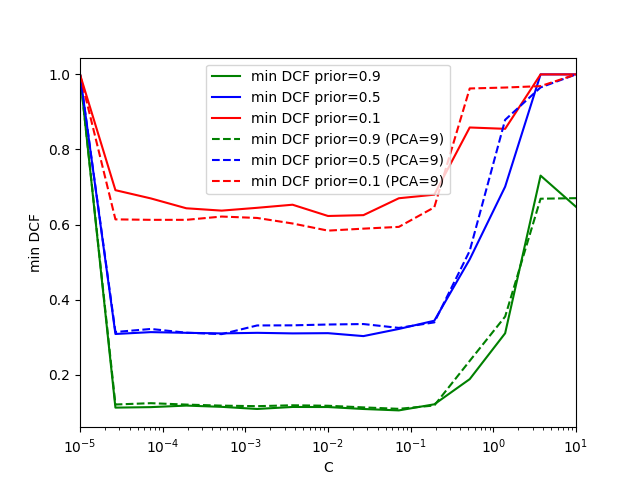
\includegraphics[scale = 0.5]{../../images/validation/SVM_Poly_minDCF_comparison_K=1_c=1_d=2}
    \centering
    \caption{Poly K=1, c=1, d=2}
    \label{fig:PolySVM_d2_valid}
\end{figure}

Figure~\ref{fig:PolySVM_d2_valid} shows the different values of C with K=1, c=1 e d=2.
We are going to try \(C = [0.01,0.1,1,10]\), but from the plot it's easy to see that C=1 and C=10 won't be good.

\begin{figure}[h!]
    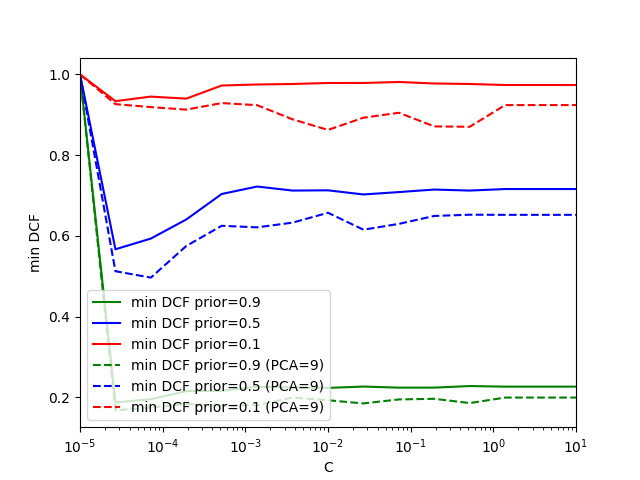
\includegraphics[scale = 0.5]{../../images/validation/SVM_Poly_minDCF_comparison_K=1_c=1_d=3}
    \centering
    \caption{Poly K=1, c=1, d=3}
    \label{fig:PolySVM_d3_valid}
\end{figure}

Figure~\ref{fig:PolySVM_d3_valid} shows the different values of C with K=1, c=1 but d=3.
It's much worse than using d=2, so we decided to don't even show the results of this kernel.
\newpage
\textbf{SVM - Quadratic - Raw Feature with degree = 2}

\begin{table}[H]
    \centering
    \begin{tabular}{ll|lllll}
        \hline
                                &  $\textbf{Constant = 0}$       & K = 0.1 & K = 1.0 & K = 10 \\ \hline
                                & & \multicolumn{3}{c}{$\pi$=0.1} \\ \hline
                                & C = 0.01   & 0.71 & 0.704 & 0.682    \\
                                & C = 0.1    & 0.713 & 0.674 & 0.678  \\
                                & C = 1.0    & 0.831 & 0.922 & 0.84    \\
                                & C = 10.0   & 0.982 & 0.994 & 0.975  \\ \hline

                                & & \multicolumn{3}{c}{$\pi$=0.5} \\ \hline
                                & C = 0.01   & 0.337 & 0.346 & \color{red}{0.342}   \\
                                & C = 0.1    & \color{red}{0.324} & \color{red}{0.344} & 0.346  \\
                                & C = 1.0    & 0.528 & 0.551 & 0.49    \\
                                & C = 10.0   & 0.947 & 0.957 & 0.946  \\ \hline

                                & & \multicolumn{3}{c}{$\pi$=0.9} \\ \hline
                                & C = 0.01   & 0.123 & 0.121 & 0.187  \\
                                & C = 0.1    & 0.125 & 0.11 & 0.115  \\
                                & C = 1.0    & 0.21 & 0.203 & 0.223    \\
                                & C = 10.0   & 0.586 & 0.769 & 0.583  \\ 
    \hline
    \end{tabular}
    \label{tab:PolySVM_c0_valid}
\end{table}

\begin{table}[H]
    \centering
    \begin{tabular}{ll|lllll}
        \hline
                                & $\textbf{Constant = 1}$      & K = 0.1 & K = 1.0 & K = 10 \\ \hline
                                & & \multicolumn{3}{c}{$\pi$=0.1} \\ \hline
                                & C = 0.01   & 0.63 & 0.623 & 0.598    \\
                                & C = 0.1    & 0.66 & 0.624 & 0.677  \\
                                & C = 1.0    & 0.96 & 0.931 & 0.95    \\
                                & C = 10.0   & 0.996 & 1.0 & 1.0  \\ \hline

                                & & \multicolumn{3}{c}{$\pi$=0.5} \\ \hline
                                & C = 0.01   & \color{red}{0.316} & \color{red}{0.311} & \color{red}{0.313}   \\
                                & C = 0.1    & 0.348 & 0.347 & 0.323  \\
                                & C = 1.0    & 0.701 & 0.631 & 0.644    \\
                                & C = 10.0   & 0.966 & 1.0 & 1.0  \\ \hline

                                & & \multicolumn{3}{c}{$\pi$=0.9} \\ \hline
                                & C = 0.01   & 0.113 & 0.114 & 0.104  \\
                                & C = 0.1    & 0.114 & 0.112 & 0.11  \\
                                & C = 1.0    & 0.281 & 0.207 & 0.233    \\
                                & C = 10.0   & 0.656 & 0.647 & 0.569  \\ 
    \hline
    \end{tabular}
    \label{tab:PolySVM_c1_valid}
\end{table}

$\newline$
\textbf{SVM - Quadratic - PCA with m = 9 and degree = 2}

$\newline$
We also show the results of PCA with m = 9 (always with d=2).
From Figure~\ref{fig:PolySVM_d2_valid} we can see that using PCA = 9 or don't use it doesn't change that much.
Just for $\pi$ = 0.1 there's a slight improvement.

\begin{table}[H]
    \centering
    \begin{tabular}{ll|lllll}
        \hline
                                & $\textbf{Constant = 0}$  &         K = 0.1 & K = 1.0 & K = 10 \\ \hline
                                & & \multicolumn{3}{c}{$\pi$=0.1} \\ \hline
                                & C = 0.01   & 0.645 & 0.645 & 0.638    \\
                                & C = 0.1    & 0.659 & 0.659 & 0.656  \\
                                & C = 1.0    & 0.92 & 0.871 & 0.916    \\
                                & C = 10.0   & 1.0 & 0.985 & 0.99  \\ \hline

                                & & \multicolumn{3}{c}{$\pi$=0.5} \\ \hline
                                & C = 0.01   & \color{red}{0.33} & \color{red}{0.344} & \color{red}{0.354}   \\
                                & C = 0.1    & 0.345 & 0.345 & 0.391  \\
                                & C = 1.0    & 0.449 & 0.575 & 0.574    \\
                                & C = 10.0   & 1.0 & 0.975 & 0.951  \\ \hline

                                & & \multicolumn{3}{c}{$\pi$=0.9} \\ \hline
                                & C = 0.01   & 0.127 & 0.124 & 0.109  \\
                                & C = 0.1    & 0.125 & 0.113 & 0.125  \\
                                & C = 1.0    & 0.181 & 0.203 & 0.172    \\
                                & C = 10.0   & 0.605 & 0.66 & 0.527  \\ 
    \hline
    \end{tabular}
    \label{tab:PolySVM_PCA9_c0_valid}
\end{table}

\begin{table}[H]
    \centering
    \begin{tabular}{ll|lllll}
        \hline
                                & $\textbf{Constant = 1}$ &         K = 0.1 & K = 1.0 & K = 10 \\ \hline
                                & & \multicolumn{3}{c}{$\pi$=0.1} \\ \hline
                                & C = 0.01   & 0.576 & 0.584 & 0.59    \\
                                & C = 0.1    & 0.586 & 0.624 & 0.667  \\
                                & C = 1.0    & 0.894 & 0.992 & 0.975    \\
                                & C = 10.0   & 0.998 & 1.0 & 0.982  \\ \hline

                                & & \multicolumn{3}{c}{$\pi$=0.5} \\ \hline
                                & C = 0.01   & \color{red}{0.335} & 0.334 & \color{red}{0.306}   \\
                                & C = 0.1    & 0.35 & \color{red}{0.302} & 0.346  \\
                                & C = 1.0    & 0.688 & 0.772 & 0.56    \\
                                & C = 10.0   & 0.993 & 1.0 & 0.975  \\ \hline

                                & & \multicolumn{3}{c}{$\pi$=0.9} \\ \hline
                                & C = 0.01   & 0.118 & 0.117 & 0.105  \\
                                & C = 0.1    & 0.132 & 0.114 & 0.107  \\
                                & C = 1.0    & 0.22 & 0.236 & 0.189    \\
                                & C = 10.0   & 0.677 & 0.67 & 0.594  \\ 
    \hline
    \end{tabular}
    \label{tab:PolySVM_PCA9_c1_valid}
\end{table}

$\newline$
\textbf{SVM - Quadratic - PCA with m = 8 and degree = 2}
$\newline$
We also tried PCA with m = 8 because it's even better for some cases.

\begin{table}[H]
    \centering
    \begin{tabular}{ll|lllll}
        \hline
                                & \textbf{Constant = 0} &         K = 0.1 & K = 1.0 & K = 10 \\ \hline
                                & & \multicolumn{3}{c}{$\pi$=0.1} \\ \hline
                                & C = 0.01   & 0.624 & 0.654 & 0.666    \\
                                & C = 0.1    & 0.66 & 0.648 & 0.658  \\
                                & C = 1.0    & 0.848 & 0.989 & 0.798    \\
                                & C = 10.0   & 0.981 & 0.999 & 0.97  \\ \hline

                                & & \multicolumn{3}{c}{$\pi$=0.5} \\ \hline
                                & C = 0.01   & 0.324 & \color{red}{0.331} & 0.333   \\
                                & C = 0.1    & \color{red}{0.321} & 0.336 & \color{red}{0.317}  \\
                                & C = 1.0    & 0.593 & 0.934 & 0.494    \\
                                & C = 10.0   & 0.97 & 0.999 & 0.91  \\ \hline

                                & & \multicolumn{3}{c}{$\pi$=0.9} \\ \hline
                                & C = 0.01   & 0.127 & 0.12 & 0.113  \\
                                & C = 0.1    & 0.124 & 0.11 & 0.116  \\
                                & C = 1.0    & 0.285 & 0.359 & 0.203    \\
                                & C = 10.0   & 0.511 & 0.74 & 0.563  \\ 
    \hline
    \end{tabular}
    \label{tab:PolySVM_PCA8_c0_valid}
\end{table}

\begin{table}[H]
    \centering
    
    \begin{tabular}{ll|lllll}
        \hline
                                & \textbf{Constant = 1} &         K = 0.1 & K = 1.0 & K = 10 \\ \hline
                                & & \multicolumn{3}{c}{$\pi$=0.1} \\ \hline
                                & C = 0.01   & 0.561 & 0.541 & 0.53    \\
                                & C = 0.1    & 0.546 & 0.592 & 0.634  \\
                                & C = 1.0    & 0.985 & 0.865 & 0.98    \\
                                & C = 10.0   & 1.0 & 0.996 & 0..994  \\ \hline

                                & & \multicolumn{3}{c}{$\pi$=0.5} \\ \hline
                                & C = 0.01   & \color{red}{0.323} & 0.32 & \color{red}{0.308}   \\
                                & C = 0.1    & 0.349 & \color{red}{0.316} & 0.336  \\
                                & C = 1.0    & 0.657 & 0.649 & 0.7    \\
                                & C = 10.0   & 1.0 & 0.985 & 0.989  \\ \hline

                                & & \multicolumn{3}{c}{$\pi$=0.9} \\ \hline
                                & C = 0.01   & 0.114 & 0.108 & 0.101  \\
                                & C = 0.1    & 0.111 & 0.113 & 0.102  \\
                                & C = 1.0    & 0.262 & 0.217 & 0.211    \\
                                & C = 10.0   & 0.697 & 0.743 & 0.647  \\
    \hline
    \end{tabular}
    \label{tab:PolySVM_PCA8_c1_valid}
\end{table}

\newpage
\textbf{SVM - Radial Basis kernel Function}
$\newline$
As we introduced in the Quadratic SVM section, there's another kernel function we are going to see.
This one is called Gaussian Radial Basis Function or RBF:
\[k(x_1,x_2) = e^{-\gamma||x_1-x_2||^2}\]
where \(||x_1-x_2||^2\) represent the distance between $x_1$ and $x_2$ and the closer it is, the bigger is
the kernel, meanwhile $\gamma$ is an indicator of the width of the kernel.
If $\gamma$ is low then the kernel will be large, otherwise it will be small (if $\gamma$ $\gg$ 0 then this will be equal to 1-NN).

\begin{figure}[h!]
    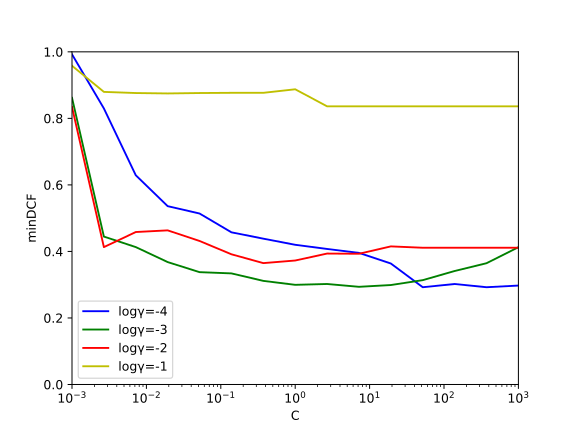
\includegraphics[scale = 0.5]{../../images/validation/SVM_RBF_minDCF_comparison}
    \centering
    \caption{RBF}
    \label{fig:RBF_valid}
\end{figure}

Figure~\ref{fig:RBF_valid} shows the different values of C with different values of $\gamma$.
We are going to test \(C = [1, 10, 100]\) with a \(\gamma = [0.001, 0.0001]\), those are the best parameter we can get.

$\newline$
\textbf{SVM - Radial Basis kernel Function - Raw Feature}
$\newline$
\begin{table}[H]
    \centering
    
    \begin{tabular}{ll|lllll}
        \hline
                                & \textbf{$\gamma$ = 0.001} &         K = 0.1 & K = 1.0 & K = 10 \\ \hline
                                & & \multicolumn{3}{c}{$\pi$=0.1} \\ \hline
                                & C = 1.0    & 0.592 & 0.575 & 0.578    \\
                                & C = 10.0   & 0.58 & 0.599 & 0.601  \\
                                & C = 100.0   & 0.586 & 0.579 & 0.601  \\ \hline

                                & & \multicolumn{3}{c}{$\pi$=0.5} \\ \hline
                                & C = 1.0    & 0.302 & 0.3 & \color{red}{0.301}    \\
                                & C = 10.0   & \color{red}{0.293} & \color{red}{0.298} & 0.302  \\
                                & C = 100.0   & 0.332 & 0.331 & 0.335  \\ \hline

                                & & \multicolumn{3}{c}{$\pi$=0.9} \\ \hline
                                & C = 1.0    & 0.097 & 0.1 & 0.101    \\
                                & C = 10.0   & 0.089 & 0.089 & 0.089  \\
                                & C = 100.0   & 0.101 & 0.103 & 0.102  \\ 
    \hline
    \end{tabular}
    \label{tab:RBF1_valid}
\end{table}


\begin{table}[H]
    \centering
    
    \begin{tabular}{ll|lllll}
        \hline
                                & \textbf{$\gamma$ = 0.0001} &         K = 0.1 & K = 1.0 & K = 10 \\ \hline
                                & & \multicolumn{3}{c}{$\pi$=0.1} \\ \hline
                                & C = 1.0    & 0.671 & 0.662 & 0.659    \\
                                & C = 10.0   & 0.574 & 0.58 & 0.584  \\
                                & C = 100.0   & 0.568 & 0.575 & 0.725  \\ \hline

                                & & \multicolumn{3}{c}{$\pi$=0.5} \\ \hline
                                & C = 1.0    & 0.473 & 0.42 & 0.419    \\
                                & C = 10.0   & 0.406 & 0.381 & \color{red}{0.354}  \\
                                & C = 100.0   & \color{red}{0.289} & \color{red}{0.306} & 0.472  \\ \hline

                                & & \multicolumn{3}{c}{$\pi$=0.9} \\ \hline
                                & C = 1.0    & 0.163 & 0.159 & 0.158    \\
                                & C = 10.0   & 0.137 & 0.133 & 0.13  \\
                                & C = 100.0   & 0.097 & 0.103 & 0.276  \\ 
    \hline
    \end{tabular}
    \label{tab:RBF2_valid}
\end{table}

$\newline$
\textbf{SVM - Radial Basis kernel Function - PCA with m=9}
$\newline$
We also tried to use PCA both with m=9 and m=8.

\begin{table}[H]
    \centering
    \begin{tabular}{ll|lllll}
        \hline
                                & \textbf{$\gamma$ = 0.001} &         K = 0.1 & K = 1.0 & K = 10 \\ \hline
                                & & \multicolumn{3}{c}{$\pi$=0.1} \\ \hline
                                & C = 1.0    & 0.588 & 0.585 & 0.579    \\
                                & C = 10.0   & 0.534 & 0.541 & 0.542  \\
                                & C = 100.0   & 0.678 & 0.671 & 0.906  \\ \hline

                                & & \multicolumn{3}{c}{$\pi$=0.5} \\ \hline
                                & C = 1.0    & \color{red}{0.295} & \color{red}{0.294} & \color{red}{0.298}    \\
                                & C = 10.0   & 0.297 & 0.301 & 0.299  \\
                                & C = 100.0   & 0.328 & 0.333 & 0.895  \\ \hline

                                & & \multicolumn{3}{c}{$\pi$=0.9} \\ \hline
                                & C = 1.0    & 0.103 & 0.104 & 0.104    \\
                                & C = 10.0   & 0.102 & 0.103 & 0.102  \\
                                & C = 100.0   & 0.107 & 0.108 & 0.285  \\ 
    \hline
    \end{tabular}
    \label{tab:RBF1_PCA9_valid}
\end{table}


\begin{table}[H]
    \centering
    \begin{tabular}{ll|lllll}
        \hline
                                & \textbf{$\gamma$ = 0.0001} &         K = 0.1 & K = 1.0 & K = 10 \\ \hline
                                & & \multicolumn{3}{c}{$\pi$=0.1} \\ \hline
                                & C = 1.0    & 0.672 & 0.672 & 0.662    \\
                                & C = 10.0   & 0.621 & 0.605 & 0.624  \\
                                & C = 100.0   & 0.553 & 0.502 & 0.592  \\ \hline

                                & & \multicolumn{3}{c}{$\pi$=0.5} \\ \hline
                                & C = 1.0    & 0.439 & 0.433 & 0.42    \\
                                & C = 10.0   & 0.407 & 0.391 & 0.376  \\
                                & C = 100.0  & \color{red}{ 0.301} & \color{red}{0.302} & \color{red}{0.317}  \\ \hline

                                & & \multicolumn{3}{c}{$\pi$=0.9} \\ \hline
                                & C = 1.0    & 0.165 & 0.159 & 0.16    \\
                                & C = 10.0   & 0.139 & 0.132 & 0.128  \\
                                & C = 100.0   & 0.103 & 0.106 & 0.12  \\ 
    \hline
    \end{tabular}
    \label{tab:RBF2_PCA9_valid}
\end{table}

With m=9 the results are more or less the same


$\newline$
\textbf{SVM - Radial Basis kernel Function - PCA with m=8}


\begin{table}[H]
    \centering
    \begin{tabular}{ll|lllll}
        \hline
                                & \textbf{$\gamma$ = 0.001} &         K = 0.1 & K = 1.0 & K = 10 \\ \hline
                                & & \multicolumn{3}{c}{$\pi$=0.1} \\ \hline
                                & C = 1.0    & 0.568 & 0.569 & 0.573    \\
                                & C = 10.0   & 0.528 & 0.54 & 0.545  \\
                                & C = 100.0   & 0.664 & 0.672 & 0.666  \\ \hline

                                & & \multicolumn{3}{c}{$\pi$=0.5} \\ \hline
                                & C = 1.0    & 0.297 & 0.297 & 0.296    \\
                                & C = 10.0   & \color{red}{0.281} & \color{red}{0.29} & \color{red}{0.294}  \\
                                & C = 100.0   & 0.318 & 0.315 & 0.305  \\ \hline

                                & & \multicolumn{3}{c}{$\pi$=0.9} \\ \hline
                                & C = 1.0    & 0.102 & 0.104 & 0.105    \\
                                & C = 10.0   & 0.101 & 0.103 & 0.103  \\
                                & C = 100.0   & 0.108 & 0.105 & 0.104  \\ 
    \hline
    \end{tabular}
    \label{tab:RBF1_PCA8_valid}
\end{table}


\begin{table}[H]
    \centering
    \begin{tabular}{ll|lllll}
        \hline
                                & \textbf{$\gamma$ = 0.0001} &         K = 0.1 & K = 1.0 & K = 10 \\ \hline
                                & & \multicolumn{3}{c}{$\pi$=0.1} \\ \hline
                                & C = 1.0    & 0.665 & 0.662 & 0.645    \\
                                & C = 10.0   & 0.617 & 0.607 & 0.679  \\
                                & C = 100.0   & 0.55 & 0.529 & 0.844  \\ \hline

                                & & \multicolumn{3}{c}{$\pi$=0.5} \\ \hline
                                & C = 1.0    & 0.439 & 0.433 & 0.43    \\
                                & C = 10.0   & 0.397 & 0.389 & \color{red}{0.387}  \\
                                & C = 100.0   & \color{red}{0.306} & \color{red}{0.29} & 0.686  \\ \hline

                                & & \multicolumn{3}{c}{$\pi$=0.9} \\ \hline
                                & C = 1.0    & 0.165 & 0.158 & 0.156    \\
                                & C = 10.0   & 0.141 & 0.135 & 0.153  \\
                                & C = 100.0   & 0.106 & 0.107 & 0.301  \\ 
    \hline
    \end{tabular}
    \label{tab:RBF2_PCA8_valid}
\end{table}
Also with m=8 the results are more or less the same

\clearpage

\section{Gaussian Mixture Models}

$\newline$
This is the last model we are going to consider.
It's a generative model and it's called Gaussian Mixture Model.
We are going to consider 4 models of GMM:
\begin{itemize}
    \item Full covariance matrix
    \item Diagonal covariance matrix
    \item Full Tied covariance matrix
    \item Diagonal Tied covariance matrix
\end{itemize}

The GMM is a distribution whose parameters are (M,S,W) where:
\[M = [\mu_1, \mu_2, \dots, \mu_K], S = [\Sigma_1, \Sigma_2, \dots, \Sigma_K],
W = [w_1, w_2, \dots, w_K]\]
The GMM density can be rapresented as:
\[f_X(x) = \sum_{c=1}^{K}\pi_c\mathcal{N} (x|\mu_c,\Sigma_c)\]

\begin{figure}[h!]
    \begin{subfigure}{0.4\textwidth}
        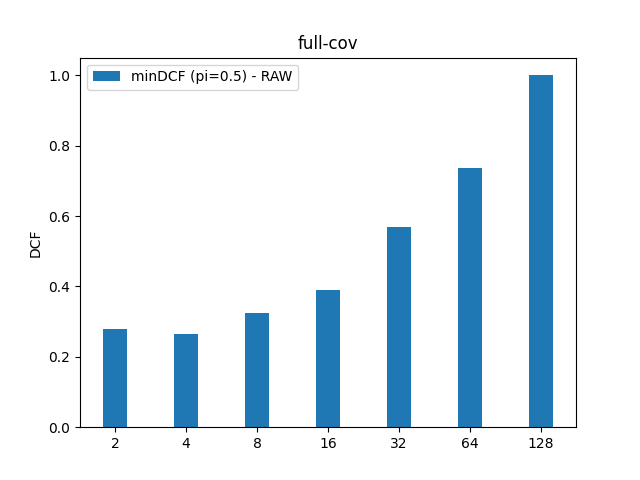
\includegraphics[scale=0.4]{../../images/validation/GMM_full-cov_component_comparison}
        \caption{GMM Full Cov}
    \end{subfigure}
    \begin{subfigure}{0.4\textwidth}
        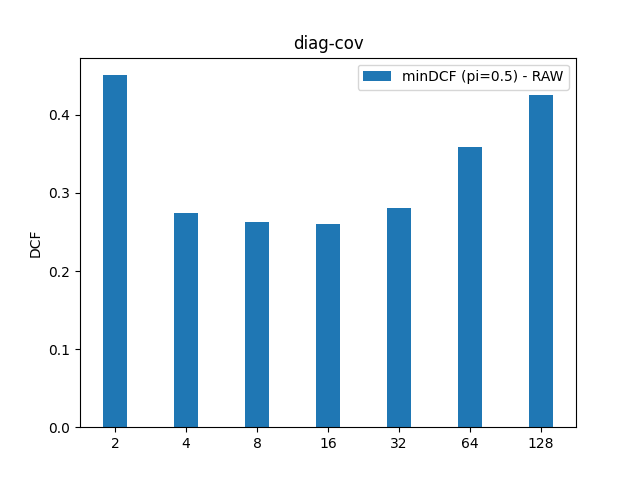
\includegraphics[scale=0.4]{../../images/validation/GMM_diag-cov_component_comparison}
        \caption{GMM Diag Cov}
    \end{subfigure}
    \begin{subfigure}{0.4\textwidth}
        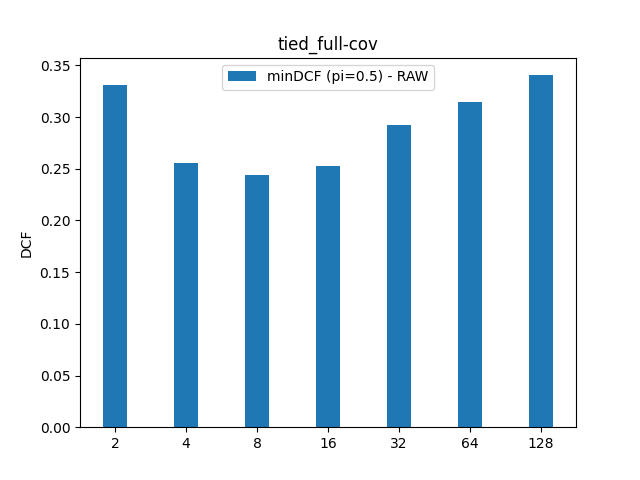
\includegraphics[scale=0.4]{../../images/validation/GMM_tied-full-cov_component_comparison}
        \caption{GMM Tied Full Cov}
    \end{subfigure}
    \begin{subfigure}{0.4\textwidth}
        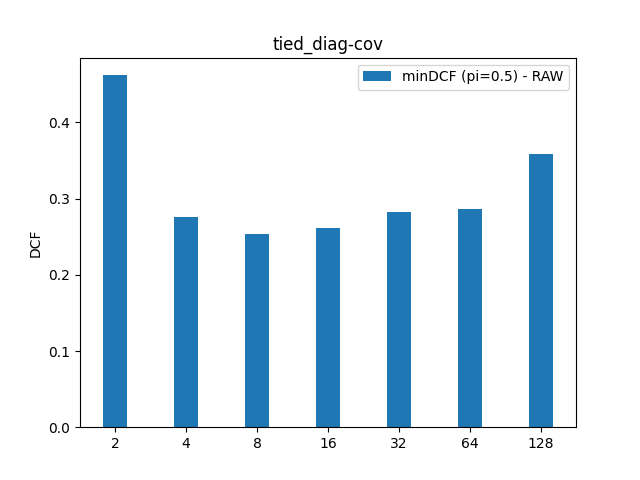
\includegraphics[scale=0.4]{../../images/validation/GMM_tied-diag-cov_component_comparison}
        \caption{GMM Tied Full Cov}
    \end{subfigure}
    \centering
    \caption{GMM with $\pi$=0.5 RAW Features}
    \label{fig:GMM_valid}
\end{figure}

Figure~\ref{fig:GMM_valid} shows the different values of minDCF with $\pi$ = 0.5 and the corresponding number
of components for each type of GMM. For example, we can see that for the full cov, the best number of
components is 4.
Here below we are going to see the results of the RAW Features and with PCA with m = 9.

$\newline$
\textbf{GMM - RAW Feature}

\begin{table}[H]
    \centering
    \begin{tabular}{ll|lllllll}
        \hline
                                & \textbf{Components} & $2$ & $4$ & $8$ & $16$ & $32$ & $64$ & $128$ \\ \hline
                                & & \multicolumn{7}{c}{$\pi$=0.1} \\ \hline
                                & Full-Cov        & 0.497 & 0.526 & 0.69 & 0.63 & 0.877 & 0.976 & 1.0   \\
                                & Diag-Cov        & 0.719 & 0.544 & 0.514 & 0.531 & 0.592 & 0.698 & 0.741  \\
                                & Full-Cov-Tied   & 0.616 & 0.611 & 0.558 & 0.542 & 0.588 & 0.563 & 0.71  \\ 
                                & Diag-Cov-Tied   & 0.805 & 0.558 & 0.501 & 0.56 & 0.601 & 0.673 & 0.765  \\ \hline

                                & & \multicolumn{7}{c}{$\pi$=0.5} \\ \hline
                                & Full-Cov          & \color{red}{0.28} & 0.264 & 0.325 & 0.391 & 0.568 & 0.737 & 1.0     \\
                                & Diag-Cov          & 0.451 & 0.275 & 0.262 & 0.26 & \color{red}{0.281} & 0.359 & 0.425  \\
                                & Full-Cov-Tied     & 0.331 & \color{red}{0.255} & \color{red}{0.244} & \color{red}{0.253} & 0.292 & 0.314 & \color{red}{0.341}  \\ 
                                & Diag-Cov-Tied     & 0.462 & 0.276 & 0.254 & 0.262 & 0.282 & \color{red}{0.286} &  0.358 \\ \hline

                                & & \multicolumn{7}{c}{$\pi$=0.9} \\ \hline
                                & Full-Cov          & 0.105 & 0.094 & 0.108 & 0.124 & 0.213 & 0.306 & 0.523    \\
                                & Diag-Cov          & 0.141 & 0.087 & 0.09 & 0.092 & 0.107 & 0.122 & 0.144  \\
                                & Full-Cov-Tied     & 0.111 & 0.098 & 0.083 & 0.087 & 0.104 & 0.108 & 0.134  \\ 
                                & Diag-Cov-Tied     & 0.144 & 0.086 & 0.089 & 0.088 & 0.093 & 0.11 & 0.131  \\ \hline 
    \hline
    \end{tabular}
    \label{tab:GMM_valid}
\end{table}

$\newline$
We can see that the Tied Full Covariance is the best in almost all components.
Meanwhile, the worst is the Full Covariance that reaches a midDCF = 1.0 with 128 components.

$\newline$
\textbf{GMM - PCA with m = 9}


\begin{table}[H]
    \centering
    \begin{tabular}{ll|lllllll}
        \hline
                                & \textbf{Components} & $2$ & $4$ & $8$ & $16$ & $32$ & $64$ & $128$ \\ \hline
                                & & \multicolumn{7}{c}{$\pi$=0.1} \\ \hline
                                & Full-Cov          & 0.455 & 0.599 & 0.599 & 0.684 & 0.837 & 0.999 & 1.0    \\
                                & Diag-Cov          & 0.742 & 0.599 & 0.553 & 0.546 & 0.513 & 0.638 & 0.729  \\
                                & Full-Cov-Tied     & 0.629 & 0.608 & 0.56 & 0.56 & 0.494 & 0.522 & 0.589  \\ 
                                & Diag-Cov-Tied     & 0.741 & 0.554 & 0.528 & 0.538 & 0.554 & 0.58 & 0.624  \\ \hline

                                & & \multicolumn{7}{c}{$\pi$=0.5} \\ \hline
                                & Full-Cov          & \color{red}{0.299} & 0.293 & 0.322 & 0.371 & 0.467 & 0.704 & 1.0    \\
                                & Diag-Cov          & 0.367 & 0.272 & 0.253 & 0.281 & 0.287 & 0.34 & 0.374  \\
                                & Full-Cov-Tied     & 0.33 & \color{red}{0.261} & 0.269 & \color{red}{0.254} & \color{red}{0.285} & \color{red}{0.324} & \color{red}{0.322}  \\ 
                                & Diag-Cov-Tied     & 0.368 & 0.268 & \color{red}{0.248} & 0.276 & 0.306 & 0.328 & 0.359  \\ \hline

                                & & \multicolumn{7}{c}{$\pi$=0.9} \\ \hline
                                & Full-Cov          & 0.099 & 0.091 & 0.113 & 0.125 & 0.158 & 0.218 & 0.376   \\
                                & Diag-Cov          & 0.114 & 0.096 & 0.094 & 0.093 & 0.103 & 0.109 & 0.135 \\
                                & Full-Cov-Tied     & 0.109 & 0.103 & 0.087 & 0.095 & 0.109 & 0.119 & 0.138  \\ 
                                & Diag-Cov-Tied     & 0.114 & 0.087 & 0.095 & 0.09 & 0.093 & 0.101 &  0.12 \\ \hline 
    \hline
    \end{tabular}
    \label{tab:GMM_PCA9_valid}
\end{table}


\clearpage
\section{Recap}
We are now going to compare three models with their best parameters: 
\begin{itemize}
    \item Multivariate Gaussian Model, \textbf{PCA m = 9}
    \item Radial Basis Function SVM, \textbf{PCA m = 8, C = 10, K = 0.1, $\gamma$ = 0.001}
    \item Gaussian Mixture Model, \textbf{RAW, Components = 8}
\end{itemize}
\textit{NOTE: we didn't considered LR beacuse it computes linear separation, so it'd have achieved the worst
result compared to the other three.}

Now let's see the Bayes Error Plot and the ROC curve of each comparison.
We start with MVG and GMM.

\begin{figure}[h!]
    \begin{subfigure}{0.5\textwidth}
        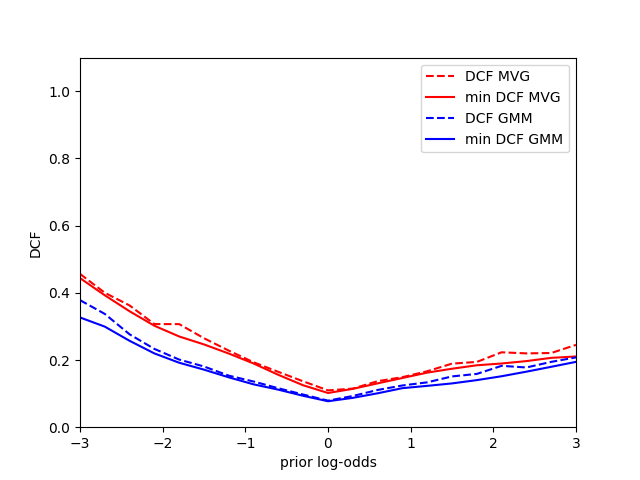
\includegraphics[scale=0.5]{../../images/comparison/validation/DCF_MVG&GMM}
    \end{subfigure}
    \begin{subfigure}{0.5\textwidth}
        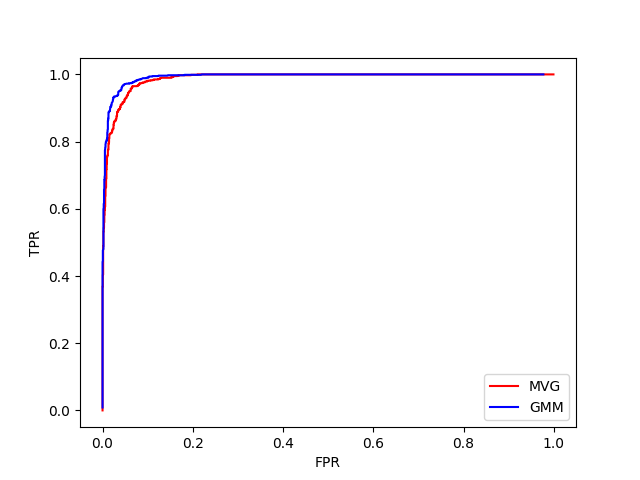
\includegraphics[scale=0.5]{../../images/comparison/validation/ROC_MVG&GMM}
    \end{subfigure}
    \label{fig:MVGvsGMM}
\end{figure}
It can be seen that GMM performs better than the MVG for both minDCF and actDCF.
Also, the actDCF of both model is close to the minDCF, so no calibration is needed.

Now let's see MVG vs SVM RBF\@.

\begin{figure}[h!]
    \begin{subfigure}{0.5\textwidth}
        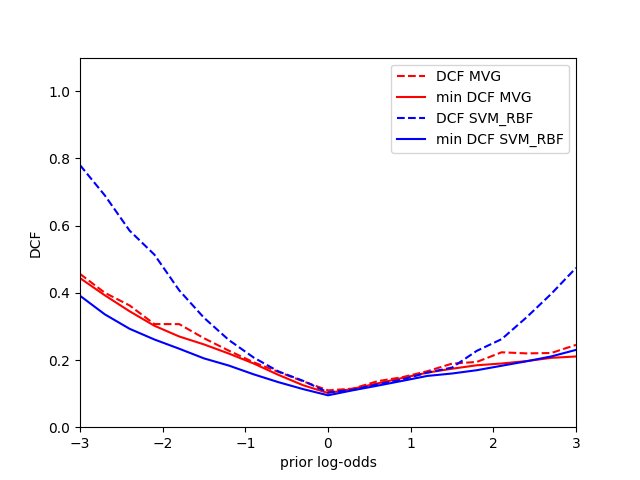
\includegraphics[scale=0.5]{../../images/comparison/validation/DCF_MVG&SVM_RBF}
    \end{subfigure}
    \begin{subfigure}{0.5\textwidth}
        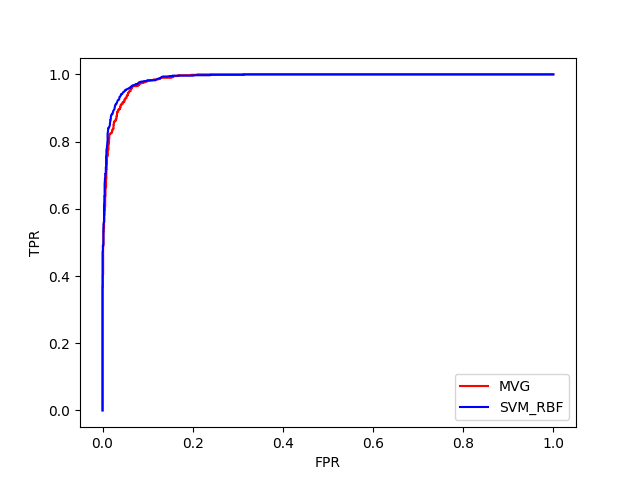
\includegraphics[scale=0.5]{../../images/comparison/validation/ROC_MVG&SVM_RBF}
    \end{subfigure}
    \label{fig:MVGvsSVM}
\end{figure}
Here we clearly need some calibration about the SVM. This is needed because the scores are not calibrated
since SVM has no probabilistic interpretation!
We are going to apply the prior weighted logistic regression as calibration model.
Let's define a function \[f(s) = \log\frac{f_{S|H}(s|H_T)}{f_{S|H}(s|H_F)} = \alpha s + \beta\]
where s is the input score, $f(s)$ computes the $s_{cal}$ that is the calibrated score.
The original score s are the scores obtained by the SVM\@.

\begin{figure}[H]
    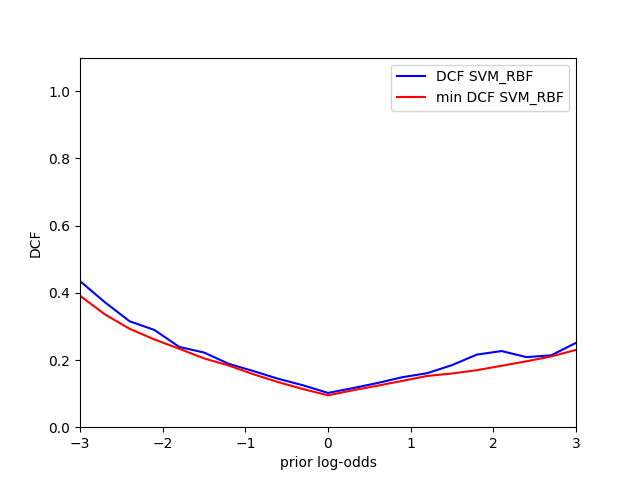
\includegraphics[scale=0.5]{../../images/comparison/validation/DCF_SVM_RBF_calibrated}
    \centering
    \caption{SVM RBF Calibrated}
    \label{fig:SVM_RBF_Cal}
\end{figure}
 Figure~\ref{fig:SVM_RBF_Cal} shows the calibrated SVM, with an actDCF that is closer to the minDCF,
 so the calibration worked.

 Now let's see the SVM RBF Calibrated vs MVG\@.
\begin{figure}[H]
    \begin{subfigure}{0.5\textwidth}
        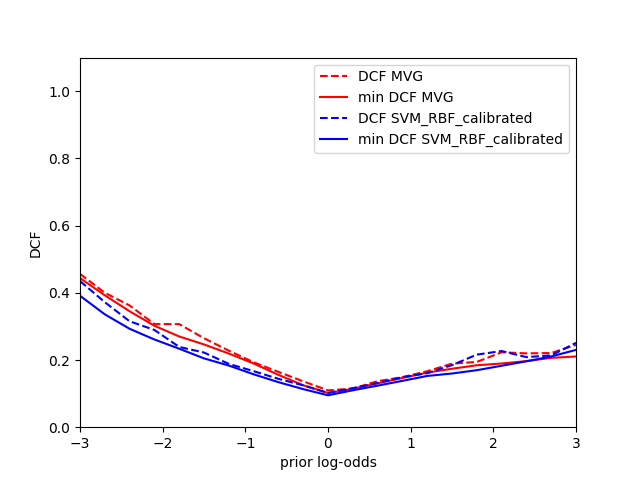
\includegraphics[scale=0.5]{../../images/comparison/validation/DCF_MVG&SVM_RBF_calibrated}
    \end{subfigure}
    \begin{subfigure}{0.5\textwidth}
        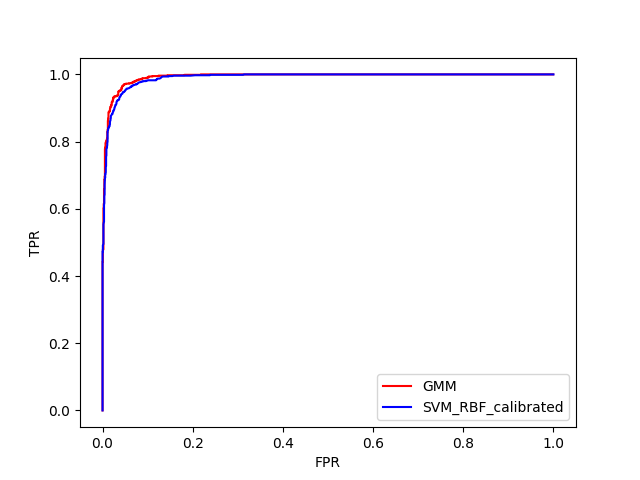
\includegraphics[scale=0.5]{../../images/comparison/validation/ROC_GMM&SVM_RBF_calibrated}
    \end{subfigure}
    \label{fig:SVMcalibvsMVG}
\end{figure}
Again the SVM RBF is slightly better than the MVG, but nothing relevant.
Last we have the comparison between the SVM RBF and GMM. Again the SVM's scores are not calibrated so let's calibrate them.

\begin{figure}[H]
    \begin{subfigure}{0.5\textwidth}
        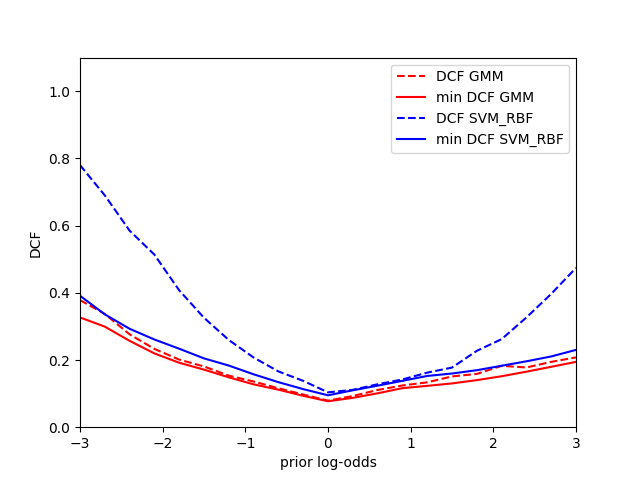
\includegraphics[scale=0.5]{../../images/comparison/validation/DCF_GMM&SVM_RBF}
    \end{subfigure}
    \begin{subfigure}{0.5\textwidth}
        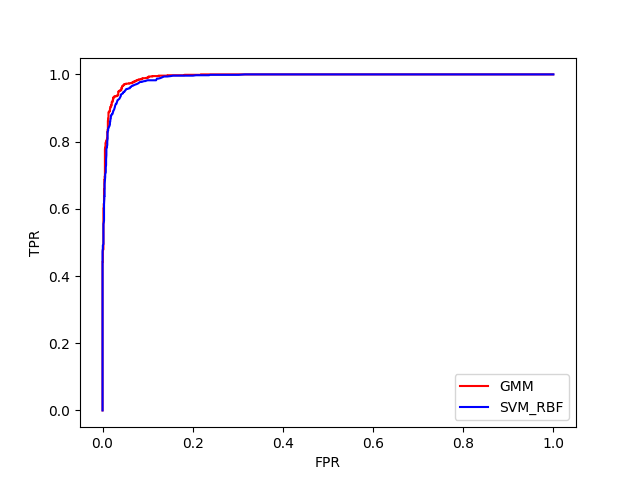
\includegraphics[scale=0.5]{../../images/comparison/validation/ROC_GMM&SVM_RBF}
    \end{subfigure}
    \label{fig:SVMvsGMM}
\end{figure}


\begin{figure}[H]
    \begin{subfigure}{0.5\textwidth}
        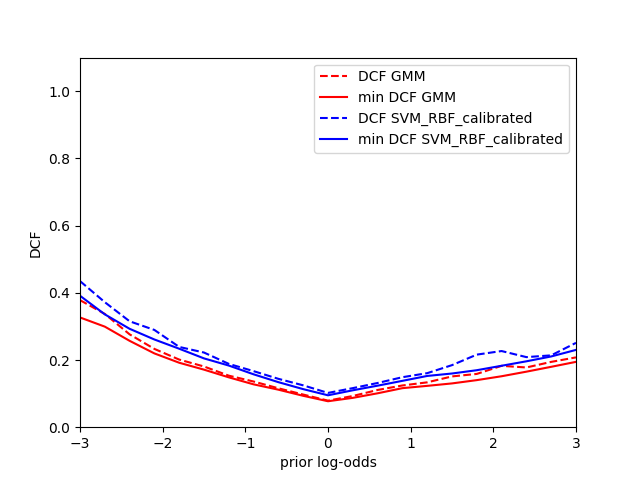
\includegraphics[scale=0.5]{../../images/comparison/validation/DCF_GMM&SVM_RBF_calibrated}
    \end{subfigure}
    \begin{subfigure}{0.5\textwidth}
        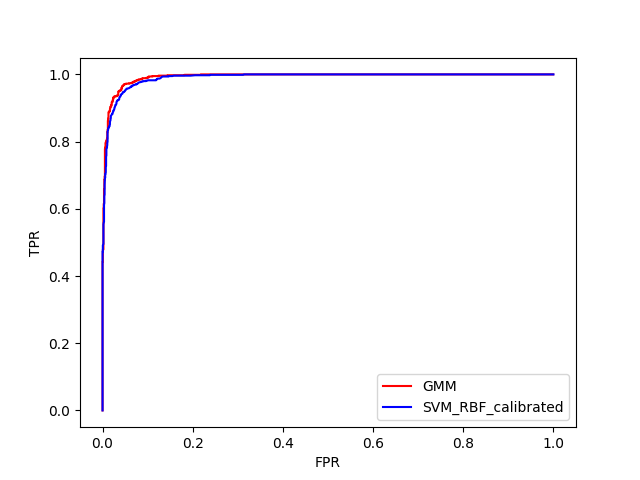
\includegraphics[scale=0.5]{../../images/comparison/validation/ROC_GMM&SVM_RBF_calibrated}
    \end{subfigure}
    \label{fig:SVMcalibvsGMM}
\end{figure}
Here we have the calibrated score, we can see that the GMM is better than the SVM\@.

$\newline$
\textbf{LAST DECISION:}
Our best model is the \textbf{Gaussian Mixture Model, RAW, Components = 8}.
Now let's use the Test set and see if the GMM is also the best model for the evaluation.



\chapter{Evaluation}

We are now going to evaluate our models using the evaluation set (or test set).
The evaluation will be done thanks to the minDCF. In the validation part we used the k-fold with k = 5, but in the evaluation part
we won't use k-fold because we don't need the validation test, since there's the test set.
So we are going to train each model on the full training set then test this model on the test set.

\section{Multivariate Gaussian Model}
In this section we are going to show the result on the \textbf{Test set} for the Gaussian part, 
exactly as we did for the validation part (that was done on the \textbf{Validation set}). We are going
to test on Raw features, PCA with m = 8 and m = 9.

\begin{table}[H]
    \centering
    \begin{tabular}{@{}llll@{}}
    \toprule
                        & pi = 0.1  & pi = 0.5  & pi = 0.9 \\ \midrule
                        & \multicolumn{3}{c}{RAW Features} \\ \midrule
    MVG                 & \color{red}{0.545}     & \color{red}{0.276}     & \color{red}{0.083}    \\
    Naive Gaussian      & 0.718     & 0.352     & 0.111    \\
    Tied Gaussian       & 0.789     & 0.455     & 0.176    \\
    Naive Tied Gaussian & 0.829     & 0.48     & 0.177    \\ \bottomrule
    \end{tabular}
    \label{tab:MVG_RAW_valid_eval}
\end{table}

\begin{table}[H]
    \centering
    \begin{tabular}{@{}llll@{}}
    \toprule
                        & pi = 0.1  & pi = 0.5  & pi = 0.9 \\ \midrule
                        & \multicolumn{3}{c}{PCA m = 9} \\ \midrule
    MVG                 & \color{red}{0.569}     & \color{red}{0.272}     & \color{red}{0.082}    \\
    Naive Gaussian      & 0.635     & 0.31      & 0.087    \\
    Tied Gaussian       & 0.783     & 0.461     & 0.177    \\
    Naive Tied Gaussian & 0.864     & 0.483     & 0.175    \\ \bottomrule
    \end{tabular}
    \label{tab:MVG_PCA9_valid_eval}
\end{table}

\begin{table}[H]
    \centering
    \begin{tabular}{@{}llll@{}}
    \toprule
                        & pi = 0.1  & pi = 0.5  & pi = 0.9 \\ \midrule
                        & \multicolumn{3}{c}{PCA m = 8} \\ \midrule
    MVG                 & \color{red}{0.571}     & \color{red}{0.271}     & \color{red}{0.083}    \\
    Naive Gaussian      & 0.638     & 0.315     & 0.087    \\
    Tied Gaussian       & 0.773     & 0.456     & 0.178    \\
    Naive Tied Gaussian & 0.865     & 0.484     & 0.176    \\ \bottomrule
    \end{tabular}
    \label{tab:MVG_PCA8_valid_eval}
\end{table}

We can see that for all 3 models (Raw, m=8, m=9) the MVG is the best.
Only for the Naive assumption the model with PCA are better than the Raw model. \newline
Comparing these results with the one obtained from the Validation part, they seem to be a little bit better, but not that much, so
the results are consistent. 

\newpage

\section{Logistic Regression}
Again, in this section there are the results for the Logistic Regression part.

\begin{figure}[h!]
    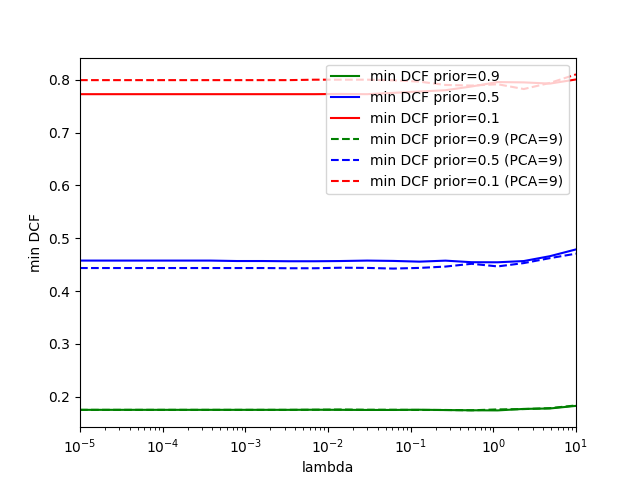
\includegraphics[scale=0.5]{../../images/evaluation/LR_PCA_minDCF_comparison}
    \centering
    \caption{LR - compare different $\lambda$}
    \label{fig:LR_eval}
\end{figure}
Figure~\ref{fig:LR_eval} shows the midDCF for each $\lambda$.
The optimal $\lambda$ = 0.4. We can also notice that for our application ($\pi$= 0.5) the model with PCA with m = 9 is slightly better.
Now let's see the results.

\begin{table}[H]
    \centering
    \begin{tabular}{lllllll}
        \toprule
               & pi=0.1 & pi=0.5 & pi=0.9 \\ \midrule
                                & \multicolumn{3}{c}{RAW Features}  \\
    Log Reg    & \color{red}{0.789}      & 0.454      & 0.175  \\ \midrule
                                & \multicolumn{3}{c}{PCA m=9}  \\
    Log Reg    & 0.79     & \color{red}{ 0.45}       & 0.175 \\ \midrule
                                & \multicolumn{3}{c}{PCA m=8}  \\
    Log Reg    & 0.789      & \color{red}{ 0.45}      & \color{red}{0.174} \\
    \bottomrule
    \end{tabular}
    \label{tab:LinearLogReg_valid_eval}
\end{table}
We can see that using the Raw or PCA models doesn't change that much, so all the three models can be considered the \("\)best\("\) choice
for LR, but for our application, from the Gaussian part, the MVG model has midDCF = \textbf{0.271}, meanwhile the best I can obtain using LR is minDCF = \textbf{0.45}.
So the LR model isn't the best choice overall.
Again, this is telling us that the linear separation isn't the one we need,
so we expect that the RBF and Poly SVM will perform better!
(In fact, those results are similar to the ones given by the Tied Gaussian, that is also linear)
By the way, the results are also consistent with the Validation part.

\newpage

\section{Support Vector Machine}
Here there are the best parameter of each SVM:
\begin{itemize}
    \item Linear SVM: K=1.0, C=1.0
    \item Quadratic SVM: K=1.0, C=0.1, degree=2, constant=1
    \item RBF SVM: K=0.1, C=10, $\gamma$=0.001
\end{itemize}

\textbf{SVM - Raw Features}

\begin{table}[H]
    \centering
    \begin{tabular}{lllll}
        \hline
                                & & $\pi$=0.1 & $\pi$=0.5 & $\pi$=0.9 \\\hline
                                
                                & Linear SVM        & 0.778 & 0.459 & 0.176 \\
                                & Quadratic SVM     & 0.529 & 0.278 & 0.098 \\
                                & RBF SVM           & 0.51  & 0.242 & 0.086\\ 
        \hline
    \end{tabular}
    \label{tab:SVM_Raw_eval}
\end{table}

\textbf{SVM - PCA with m = 9}

\begin{table}[H]
    \centering
    \begin{tabular}{lllll}
        \hline
                                & & $\pi$=0.1 & $\pi$=0.5 & $\pi$=0.9 \\\hline
                                                        
                                & Linear SVM        & 0.79  & 0.456 & 0.179 \\
                                & Quadratic SVM     & 0.541 & 0.274 & 0.093 \\
                                & RBF SVM           & 0.494 & 0.24  & 0.084\\  
        \hline
    \end{tabular}
    \label{tab:SVM_PCA9_eval}
\end{table}

\textbf{SVM - PCA with m = 8}

\begin{table}[H]
    \centering
    \begin{tabular}{lllll}
        \hline
                                & & $\pi$=0.1 & $\pi$=0.5 & $\pi$=0.9 \\\hline
                                                        
                                & Quadratic SVM     & 0.51 & 0.266 & 0.092 \\
                                & RBF SVM           & 0.469  & 0.236 & 0.084\\    
        \hline
    \end{tabular}
    \label{tab:SVM_PCA8_eval}
\end{table}

As we said, the RBF and the Quadratic that are non-linear achieve good results.
They are pretty similar to the MVG (that is also quadratic), but are way better than the linear ones, for example the LR.

\newpage

\section{Gaussian Mixture Model}
We are now going to see how GMM handles the Test set.

\begin{figure}[h!]
    \begin{subfigure}{0.4\textwidth}
        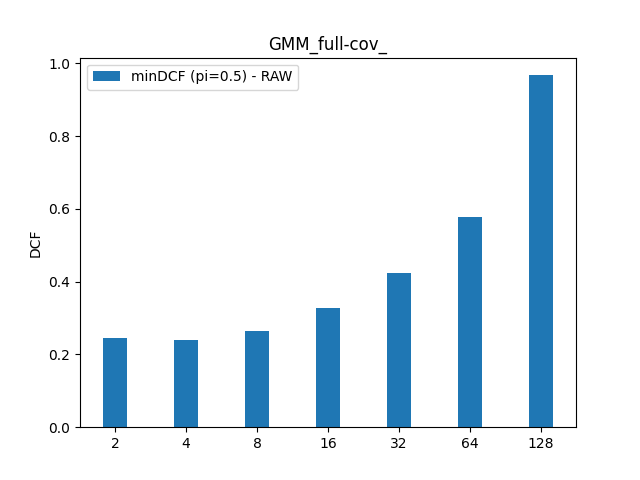
\includegraphics[scale=0.4]{../../images/evaluation/GMM_full-cov_component_comparison}
        \caption{Full Covariance}
    \end{subfigure}
    \begin{subfigure}{0.4\textwidth}
        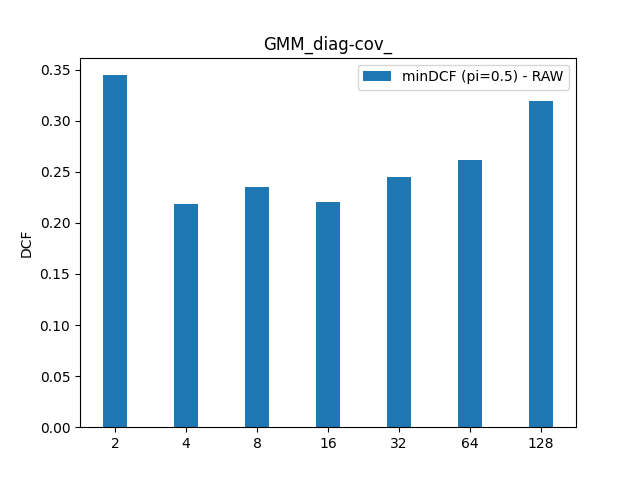
\includegraphics[scale=0.4]{../../images/evaluation/GMM_diag-cov_component_comparison}
        \caption{Diagonal Covariance}
    \end{subfigure}
    \begin{subfigure}{0.4\textwidth}
        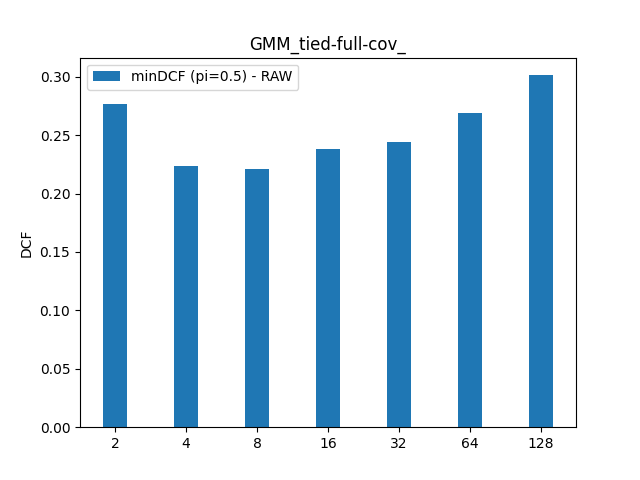
\includegraphics[scale=0.4]{../../images/evaluation/GMM_tied-full-cov_component_comparison}
        \caption{Full Tied Covariance}
    \end{subfigure}
    \begin{subfigure}{0.4\textwidth}
        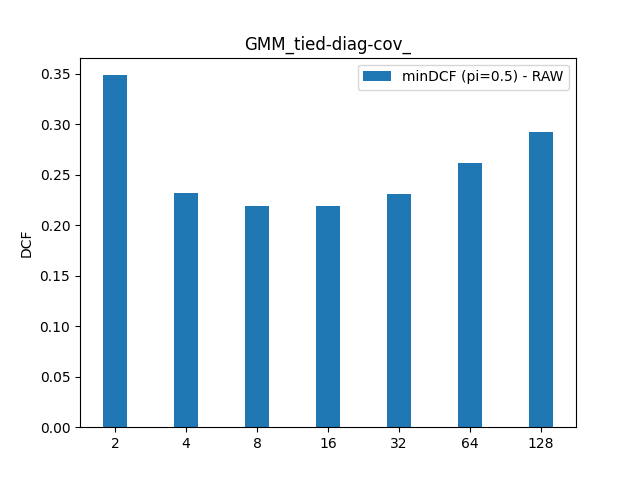
\includegraphics[scale=0.4]{../../images/evaluation/GMM_tied-diag-cov_component_comparison}
        \caption{Diagonal Tied Covariance}
    \end{subfigure}
    \centering
    \label{fig:GMM_eval}
\end{figure}
We have chosen 8 components, which seems to be the best number of components in the validation part.
\newline

\textbf{GMM - Raw Features and PCA with m = 9}
\begin{table}[H]
    \centering
    \begin{tabular}{ll|l|ll}
        \hline
                                & & RAW & PCA m = 9 \\ \hline
                                & & \multicolumn{2}{c}{$\pi$=0.1} \\ \hline
                                & Full-Cov        & 0.501  & 0.553 \\
                                & Diag-Cov        & 0.51 & \color{red}{0.467} \\
                                & Full-Cov-Tied   & 0.503 & 0.438 \\ 
                                & Diag-Cov-Tied   & 0.474 & 0.484 \\ \hline

                                & & \multicolumn{2}{c}{$\pi$=0.5} \\ \hline
                                & Full-Cov          & 0.264  & 0.268   \\
                                & Diag-Cov          & 0.235  & 0.218 \\
                                & Full-Cov-Tied     & 0.221  & \color{red}{0.217} \\ 
                                & Diag-Cov-Tied     & 0.219  & 0.226 \\ \hline

                                & & \multicolumn{2}{c}{$\pi$=0.9} \\ \hline
                                & Full-Cov          & 0.086  & 0.093  \\
                                & Diag-Cov          & 0.074  & 0.076\\
                                & Full-Cov-Tied     & 0.077  & 0.074\\ 
                                & Diag-Cov-Tied     & \color{red}{0.071}  & 0.072\\  
    \hline
    \end{tabular}
    \label{tab:GMM_RAW_eval}
\end{table}
The GMM on the Test set is again consistent with the one on the Validation set.
The best we can do for our application is with the Full Tied Covariance Matrix with minDCF = 0.217.

\newpage
\section{Recap}
As we did for the evaluation part, we are going to compare the three models:
\begin{itemize}
    \item Multivariate Gaussian Model, \textbf{PCA m = 9}
    \item Radial Basis Function SVM, \textbf{PCA m = 8, C = 10, K = 0.1, $\gamma$ = 0.001}
    \item Gaussian Mixture Model, \textbf{RAW, Components = 8}
\end{itemize}
\textit{NOTE: we didn't considered LR beacuse it computes linear separation, so it'd have achieved the worst
result compared to the other three.}

Let's start with MVG vs GMM.
\begin{figure}[H]
    \begin{subfigure}{0.5\textwidth}
        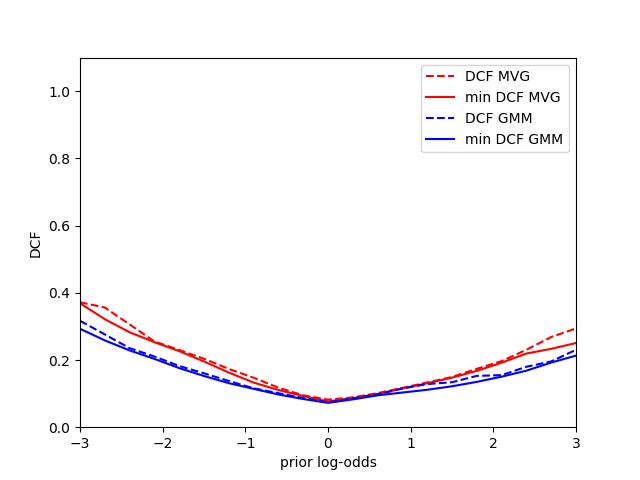
\includegraphics[scale=0.5]{../../images/comparison/evaluation/DCF_MVG&GMM}
    \end{subfigure}
    \begin{subfigure}{0.5\textwidth}
        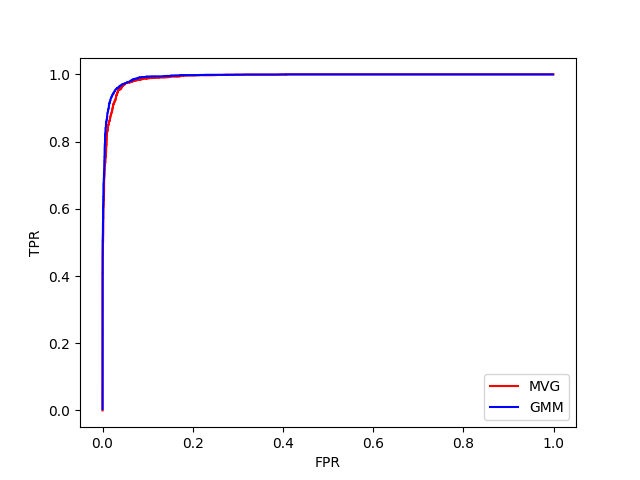
\includegraphics[scale=0.5]{../../images/comparison/evaluation/ROC_MVG&GMM}
    \end{subfigure}
    \label{fig:eval_MVGvsGMM}
\end{figure}

The minDCF and actDCF are close, so we don't need any calibration.
The GMM model is better than the MVG for both actDCF and minDCF. Now let's see the SVM vs MVG.

\begin{figure}[H]
    \begin{subfigure}{0.5\textwidth}
        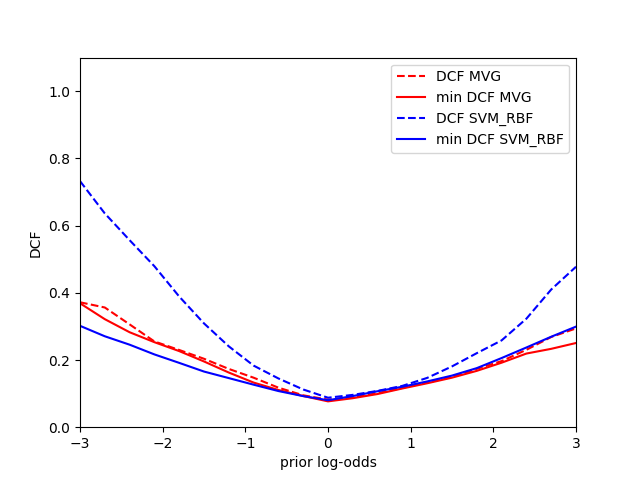
\includegraphics[scale=0.5]{../../images/comparison/evaluation/DCF_MVG&SVM_RBF}
    \end{subfigure}
    \begin{subfigure}{0.5\textwidth}
        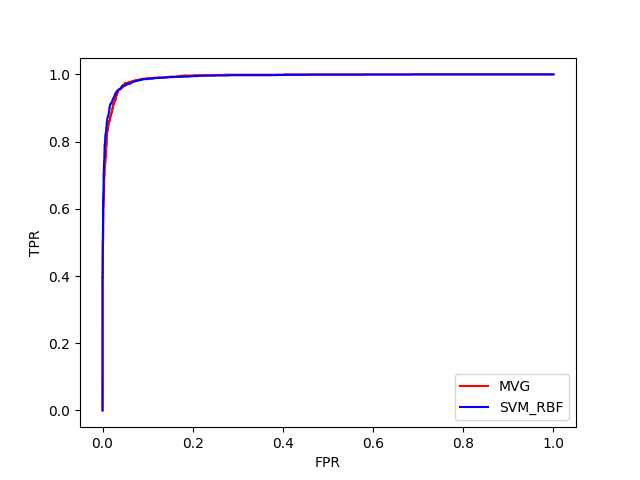
\includegraphics[scale=0.5]{../../images/comparison/evaluation/ROC_MVG&SVM_RBF}
    \end{subfigure}
    \label{fig:eval_MVGvsSVM}
\end{figure}
Again the SVM RBF is not calibrated, so we need to calibrate the scores.
We used the prior weighted logistic regression.

\begin{figure}[H]
    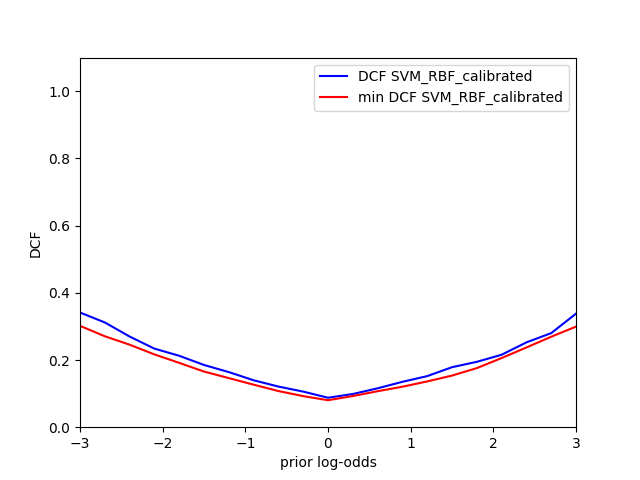
\includegraphics[scale=0.5]{../../images/comparison/evaluation/DCF_SVM_RBF_calibrated}
    \centering
    \caption{SVM RBF Calibrated}
    \label{fig:SVM_RBF_eval_cal}
\end{figure}
Figure~\ref{fig:SVM_RBF_eval_cal} shows the calibrated SVM.

\begin{figure}[H]
    \begin{subfigure}{0.5\textwidth}
        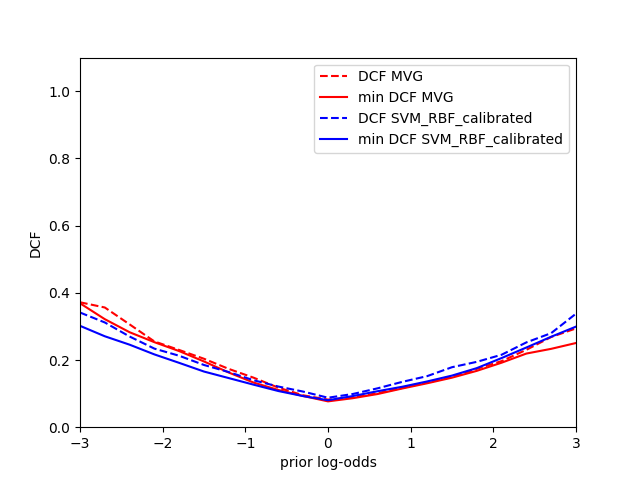
\includegraphics[scale=0.5]{../../images/comparison/evaluation/DCF_MVG&SVM_RBF_calibrated}
    \end{subfigure}
    \begin{subfigure}{0.5\textwidth}
        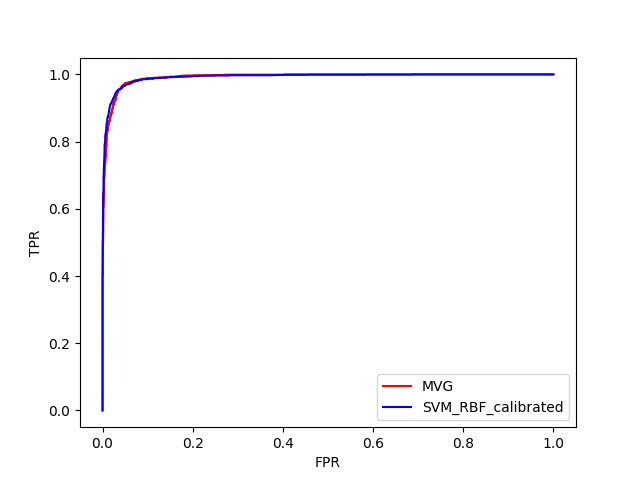
\includegraphics[scale=0.5]{../../images/comparison/evaluation/ROC_MVG&SVM_RBF_calibrated}
    \end{subfigure}
    \label{fig:eval_MVGvsSVMcalib}
\end{figure}
Here the SVM RBF calibrated vs MVG. We can see that SVM is better than the MVG. The last comparison
is between SVM RBF and GMM.

\begin{figure}[H]
    \begin{subfigure}{0.5\textwidth}
        \includegraphics[scale=0.5]{../../images/comparison/evaluation/DCF_GMM&SVM_RBF}
    \end{subfigure}
    \begin{subfigure}{0.5\textwidth}
        \includegraphics[scale=0.5]{../../images/comparison/evaluation/ROC_GMM&SVM_RBF}
    \end{subfigure}
    \label{fig:eval_GMMvsSVM}
\end{figure}
Again, the scores are not calibrated, let's calibrate them.

\begin{figure}[H]
    \begin{subfigure}{0.5\textwidth}
        \includegraphics[scale=0.5]{../../images/comparison/evaluation/DCF_GMM&SVM_RBF_calibrated}
    \end{subfigure}
    \begin{subfigure}{0.5\textwidth}
        \includegraphics[scale=0.5]{../../images/comparison/evaluation/ROC_GMM&SVM_RBF_calibrated}
    \end{subfigure}
    \label{fig:eval_GMMvsSVMcalib}
\end{figure}
We can see that the GMM is better than the SVM.

$\newline$
\textbf{Final Decision}
The best model is again the Gaussian Mixture Model with 8 components, but the with the RAW we
obtain midDCF = 0.219 and with PCA with m = 9 we obtain midDCF = 0.217.
So the best of the best would be the GMM PCA with m = 9 instead of GMM RAW. Anyway, the difference is so small that we can
consider that the expectation made on the validation part are right.





\end{document}